\documentclass[12pt,a4paper,oneside]{report}        % Single-side
%\documentclass[12pt,a4paper,twoside]{report}  		% Duplex

\usepackage[T1]{fontenc}
\usepackage[utf8]{inputenc}
\usepackage{amsmath}
\usepackage{amssymb}
\usepackage{enumerate}
\usepackage{graphicx}
\usepackage{lastpage}
\usepackage{anysize}
\newcommand\magyarOptions{chapterhead=unchanged}
\usepackage[magyar]{babel}
\usepackage{sectsty}
\usepackage{setspace}
\usepackage{hyperref}
\usepackage{fancyhdr}
\usepackage{titlesec}
\usepackage{pdfpages}
\usepackage[intoc]{nomencl}
\usepackage{lipsum}
\usepackage{float}
\usepackage{caption}
\usepackage{algorithm}
\usepackage{algpseudocode}
\usepackage[a-2b,mathxmp]{pdfx}
\usepackage{longtable}
\usepackage{url}
\usepackage{tikz}


\setlength{\parindent}{12pt}
\setlength{\parskip}{0pt}

\renewcommand{\baselinestretch}{1.5}
\titlespacing*{\section}
{0pt}{5.5ex plus 1ex minus .2ex}{4.3ex plus .2ex}

\marginsize{35.4mm}{25.4mm}{25.4mm}{25.4mm} % anysize package

\titleformat{\chapter}[display]{\fontsize{14}{15} \bfseries}{\thechapter. \chaptername}{15pt}{}
\sectionfont{\fontsize{12}{15}\bfseries}
\subsectionfont{\fontsize{12}{15}\bfseries}

\hypersetup{
	bookmarks=true,            % show bookmarks bar?
	unicode=false,             % non-Latin characters in Acrobat’s bookmarks
	pdftitle={},        % title
	pdfauthor={},    % author
	pdfsubject={}, % subject of the document
	pdfcreator={},   % creator of the document
	pdfproducer={Producer},    % producer of the document
	pdfkeywords={keywords},    % list of keywords
	pdfnewwindow=true,         % links in new window
	colorlinks=true,           % false: boxed links; true: colored links
	linkcolor=black,           % color of internal links
	citecolor=black,           % color of links to bibliography
	filecolor=black,           % color of file links
	urlcolor=black             % color of external links
}

\pagestyle{fancy}
\fancyhf{}
\fancyfoot[C]{\thepage}
\fancyhead[C]{\leftmark}

\fancypagestyle{plain}{%
	\fancyhf{}%
	\fancyfoot[C]{\thepage}%
	\fancyhead{}
	\renewcommand{\headrulewidth}{0pt}
}

\renewcommand{\chaptermark}[1]{%
	\markboth{#1}{}}
\renewcommand{\headrulewidth}{\iffloatpage{0pt}{0.4pt}}

\DeclareMathOperator*{\argmax}{arg\,max}
\DeclareMathOperator*{\argmin}{arg\,min}
%alairasok beszurasa nyilatkozatokra
\newcommand*{\SignatureAndDate}[1]{%
\par\noindent\makebox[3.5in]{}\hfill\makebox[2.0in]{\dotfill}%
\par\noindent\makebox[3.5in]{}\hfill\makebox[1.8in]{#1}
}%

\renewcommand{\nomname}{Jelölésjegyzék}

\makenomenclature
\makeindex

%%%%%%%%%%%%%%%%%%%%%%%%%%%%%%%%%%%%%%%%%%%%%%%%%%%%%%%%%%%%%%%%%%%%%%%%%%%%%%%%%%%%%%%%%%%%%%%%%%%%%
%%%%%% adatok: FONTOS, HOGY MINDEGYIK ADAT UTÁN LEGYEN SPACE! %%%%%%%%%%%%%%%%%%%%%%%%%%%%%%%%%%%%%%%
\def\myuni{Pannon Egyetem }
\def\mykar{Műszaki Informatikai Kar }
\def\mytanszek{\textbf{\textcolor{red}{<<tanszék>>}} } %többi tanszék?
\def\mycim{\textbf{\textcolor{red}{<<A szakdolgozat címe - a témakiírással egyezően>>}} }
\def\myszak{\textbf{\textcolor{red}{<<szak>>}} } %Mérnökinformatikus/Gazdaságinformatikus/Programtervező Informatikus/ Villamosmérnöki
\def\mynev{\textbf{\textcolor{red}{<<hallgató neve>>}} }
\def\myev{\textbf{\textcolor{red}{<<végzés éve>>}} }
\def\mytemavezeto{\textbf{\textcolor{red}{<<témavezető neve>>}} }
\def\mykonzulens{\textbf{\textcolor{red}{<<külső konzulens neve>>, <<intézménye>> }} }
\def\mydate{\textbf{\textcolor{red}{<<év. hónap nap>> }} }
\def\myvaros{\textbf{\textcolor{red}{<<hely>>}} }
\def\myvegzettseg{\textbf{\textcolor{red}{<<végzettség>>}} }
\def\mydolgozat{\textbf{\textcolor{red}{<<szak-/diplomadolgozat>>}} }

%%%%%%%%% kitöltendő - komment kitöRlése után ez kerül be a dolgozatba, és nem a piros fenti rész %%%%%%%%%%%%%%
%%%%%% FONTOS, HOGY MINDEGYIK ADAT UTÁN LEGYEN SPACE! %%%%%%%%%%%%%%%%%%%%%%%%%%%%%%%%%%%%%%%
%%%%%% A még nem biztos (pl pontos dátum az aláírásnál) részt érdemes még kikommentelve hagyni, így pirossal marad bent a végéig %%%%%%%%
\def\mycim{3D memóriajáték tervezése mesterséges intelligenciával }
\def\mynev{Csesznák Tamás Levente }
\def\myev{2024 }
\def\mytemavezeto{Szabó Patrícia }
%\def\mykonzulens{<<külső konzulens neve>>, <<intézménye>> }
\def\mydate{2024.05.01 }
\def\myvaros{Veszprém }


%%%%%%%%% tanszék - megfelelő elől kivenni a kommentet %%%%%%%%%%%%%%%%%%%%%%%
%\def\mytanszek{Alkalmazott Informatikai }
\def\mytanszek{Informatikai Rendszerek és Alkalmazásai }
%\def\mytanszek{Matematika }
%\def\mytanszek{Rendszer- és Számítástudományi }
%\def\mytanszek{Villamosmérnöki és Információs Rendszerek }


%%%%%%%%% szakok - megfelelő elől kivenni a kommentet %%%%%%%%%%%%%%%%%%%%%%%%%%%%%%%%%%%%
    %% Gazdaságinformatikus BSc
%\def\myszak{Gazdaságinformatikus BSc} \def\myvegzettseg{gazdaságinformatikus } \def\mydolgozat{SZAKDOLGOZAT}
    
    %% Mérnökinformatikus BSc
\def\myszak{Mérnökinformatikus BSc} \def\myvegzettseg{mérnökinformatikus } \def\mydolgozat{SZAKDOLGOZAT}
    
    %% Programtervező informatikus BSc
%\def\myszak{Programtervező informatikus BSc} \def\myvegzettseg{programtervező informatikus } \def\mydolgozat{SZAKDOLGOZAT}

    %% Villamosmérnöki BSc
%\def\myszak{Villamosmérnöki BSc} \def\myvegzettseg{villamosmérnöki } \def\mydolgozat{SZAKDOLGOZAT}

    %% Mérnökinformatikus MSc
%\def\myszak{Mérnökinformatikus MSc} \def\myvegzettseg{okleveles mérnökinformatikus } \def\mydolgozat{DIPLOMADOLGOZAT}

    %% Programtervező informatikus MSc
%\def\myszak{Programtervező informatikus MSc} \def\myvegzettseg{okleveles programtervező informatikus } \def\mydolgozat{DIPLOMADOLGOZAT}




%itt kerülnek becsatolásra a dolgozat egymást követő fejezetei
\begin{document}
	\pagenumbering{arabic}
	\onehalfspacing
	%a fedlappal kezdj
	%\begin{titlepage}
%    \begin{center}
%        \vspace*{\fill}
%        \Huge \textbf{SZAKDOLGOZAT}\\
%        \vspace{10cm}
%        \Large \textbf{Gyurácz Olivér}\\
%        \vspace{1.5cm}
%        \large 2021
%        \vspace*{\fill}
%    \end{center}
%\end{titlepage}
\begin{titlepage}
    \begin{center}
        \vspace*{\fill}
        \large \textbf{\myuni}\\
        \large \mykar\\
        \large \mytanszek Tanszék\\
        \large \myszak \\
        \vspace{2cm}
        \Huge \textbf{\mydolgozat}\\
        \vspace{2cm}
        %a szakdolgozat címe
        \Large \textbf{\mycim}\\
        \vspace{2cm}
        %a dolgozatot készítő hallgató neve
        \Large \textbf{\mynev}\\
        \vspace{2cm}
        %témavezetőjének a neve
        \large Témavezető: \mytemavezeto\\
        \vspace{1cm}
        %ha van, akkor kitöltendő, ha nincs, akkor törölje a következő sort
        %\large Külső/belső konzulens: \mykonzulens\\
        \vspace{1cm}
        % a dolgozat készítésének évszáma
        \large \myev
        \vspace*{\fill}
    \end{center}
\end{titlepage} 
	%a szkennelt témakiírás a következő, amit pdf-ben csatolunk
	
\includepdf{Temakiiras.pdf}
	%saját nyilatkozatod nyomtatva, aláírva, pdf-be szkennelve csatolandó. A szerkeszthető részt tartalmazó  h_nyilatkozat.tex fájlt nem kell becsatolni, miután az aláírt nyilatkozat csatolásra kerül
	\begin{center}
\textbf{\large{Hallgatói nyilatkozat}}\\[32pt]
\end{center}

\thispagestyle{fancy}
\pagestyle{fancy}
Alulírott \mynev (Neptun kód: \myneptun ) hallgató kijelentem, és a dolgozat feltöltésével egyidejűleg nyilatkozom, hogy a \mycim című \mydolgozategy  (a továbbiakban: dolgozat) a \myuni \mytanszek Tanszékén készítettem a \myvegzettseg oklevél megszerzése érdekében.\par

Kijelentem, hogy a dolgozatban csak a megadott és hivatkozott forrásokat használtam fel, és ezekre a vonatkozó idézési szabályok szerint hivatkoztam.
\vspace{0.6cm}\par

Nyilatkozom, hogy a dolgozat érdemi része saját szellemi alkotásom eredménye, és azt más intézményben, szakon, vagy felsőfokú képesítés megszerzésére nem nyújtottam be. Tudomásul veszem, hogy a plágium vagy szerzői jogsértés esetén a dolgozatom elutasításra kerülhet, és ellenem fegyelmi eljárás indulhat. Tudomásul veszem továbbá, hogy szerzői jogsértés esetén az Egyetem jogosult a dolgozat elérhetőségét korlátozni, valamint eltávolítani a dokumentumot a dolgozatok tárolására szolgáló, a témát vezető szervezeti egység által meghatározott elektronikus zárt rendszerből.
\vspace{0.6cm}\par

Tudomásul veszem továbbá, hogy a Pannon Egyetem a dolgozat eredményeit saját céljaira eltérő írásbeli megállapodás hiányában a Pannon Egyetem Szellemi Tulajdon Kezelési Szabályzatában foglaltaknak megfelelően szabadon felhasználhatja. 
Nyilatkozom, hogy a dolgozat elkészítése során mesterséges intelligencia eszközöket \myMIstatement. 
\vspace{0.6cm}\par


Nyilatkozom, hogy a dolgozat elkészítése során az alábbi táblázatban feltüntetett mesterséges intelligencia eszközöket kizárólag a kutatási, illetve fejlesztési feladat támogatására használtam fel, az érdemi munka, elemzés és következtetések teljes mértékben saját szellemi alkotásomat képezik.\\

%%%ha nem használtál AI-t, a következő sort vedd ki:
A dolgozatban felhasznált mesterséges intelligencia használatot részletező táblázat:\par
\begin{table}[htb!]
\centering
\arrayrulecolor{black}
\begin{tabular}{!{\color{black}\vrule}>{\hspace{0pt}}m{0.24\linewidth}!{\color{black}\vrule}>{\hspace{0pt}}m{0.31\linewidth}!{\color{black}\vrule}>{\hspace{0pt}}m{0.187\linewidth}!{\color{black}\vrule}>{\hspace{0pt}}m{0.160\linewidth}!{\color{black}\vrule}} 
\hline
\textbf{Alkalmazott technológia} & \textbf{Alkalmazás módja} & \textbf{Előállított tartalom} & \textbf{MI használat aránya} \\ 
\hline
ChatGPT o1-preview (OpenAI)  & Angol fordítás & Abstract & 90\% \\ 
\hline
ChatGPT 4o (OpenAI) & Szöveg generálása: tartalmi összefoglaló & 3. fejezet & 70\% \\ 
\hline
ChatGPT 4o (OpenAI) & Kód generálása & Node.js fájl szerver alapjai & 40\% \\ 
\hline
ChatGPT 4o (OpenAI) & Python kód generálása & Flask webszerver alapjai & 70\% \\ 
\hline
ChatGPT 4o (OpenAI) & Python kód generálása & TensorFlow használata & 30\% \\ 
\hline
ChatGPT 4o (OpenAI) & Nyelvi Stilizálás & Teljes dolgozat & 20\% \\ 
\hline
\end{tabular}
\arrayrulecolor{black}
\end{table}




\vspace{2cm}
Dátum: \myvaros, \mydate\\
\vspace{2cm}

\SignatureAndDate{\mynev}

	%\includepdf{Hallgatoi_nyilatkozat.pdf}
	%témavezetőd nyilatkozata nyomtatva, aláírva, pdf-be szkennelve csatolandó. A szerkeszthető oldalt ki kell kapcsolni majd, ha a szkennelt témavezetői nyilatkozatot beszúrta. A beszúráshoz vegye le a % jelet a 94-es és 98-as sorok elől.
	\begin{center}
\textbf{\large{Témavezetői nyilatkozat}}\\[32pt]
\end{center}

\thispagestyle{fancy}
\pagestyle{fancy}
Alulírott \mytemavezeto témavezető kijelentem, hogy a dolgozatot \mynev a \myuni \mytanszek Tanszékén készítette a \myvegzettseg végzettség megszerzése érdekében.\\

Kijelentem, hogy a dolgozat védésre bocsátását engedélyezem.\\



\vspace{2cm}
Dátum: \myvaros, \mydate\\
\vspace{2cm}

\SignatureAndDate{\mytemavezeto}

	%
\includepdf{Temavezetoi_nyilatkozat.pdf}
	%köszönetnyilvánítás csatolása
	\textbf{\large{Köszönetnyilvánítás}}\\[32pt]

\thispagestyle{fancy}
\pagestyle{fancy}

Dolgozatom elkészültével szeretnék köszönetet mondani .....2-3 mondatban megfogalmazva.\\

Ezen kívül szeretnék köszönetet mondani e .. további köszönet akinek szeretné a Hallgató kifejezni.\\

Végül szeretném megköszönni a családomnak és a barátaimnak, amiért mindvégig önzetlenül támogattak célom elérésében.\\
\\

	%tartalmi összefoglalók csatolása, ami magyar és angol nyelven az Abstract.tex fájlban lesz megírva
	\textbf{\large{Tartalmi összefoglaló}}\\[32pt]

\thispagestyle{fancy}
\pagestyle{fancy}



\vspace{8pt}

Tartalmi összefoglaló magyarul. Az összefoglalónak tartalmaznia kell (rövid, velős és összefüggő megfogalmazásban) a következőket:
\begin{itemize}
    \item téma megnevezése,
    \item megoldott feladat megfogalmazása,
    \item megoldási mód,
    \item elért eredmények,
    \item kulcsszavak (4-6 darab).
\end{itemize}
A tartalmi összefoglaló terjedelme nem lehet több egy A4-es oldalnál.\par
Az összefoglalót magyar és angol nyelven kell készíteni. Sorrendben a dolgozat nyelvével megegyező kerül előrébb. A cím Title stílusú, formázása: Times New Roman/ Computer Modern, nagybetű, 14 pt, félkövér, középre igazított; az összefoglaló szövege Normál stílusú, formázása: Times New Roman, 12 pt, sorkizárt, 1.5-ös sortávolság.

\vspace{8pt}



\textbf{Kulcsszavak: } Kulcsszó1, kulcsszó2, kulcsszó3, kulcsszó4, kulcsszó5, kulcszó6

\newpage



\textbf{\large{Abstract}}\\[32pt]

\thispagestyle{fancy}
\pagestyle{fancy}

\vspace{8pt}

Tartalmi összefoglaló angol nyelven, a tartalma és formázása megegyezik a magyar nyelvű tartalmi összefoglalóval.

\vspace{8pt}


\textbf{Keywords: } Keyword1, Keyword2, Keyword3, Keyword4, Keyword5, Keyword6 
	%Tartalomjegyzéket a Tex generálja, nem kell szerkeszteni
	\tableofcontents\vfill
	\addtocontents{toc}{\protect\thispagestyle{empty}}
	\pagestyle{empty}
	%rövidítések jegyzése a Jelolesjegyzek.tex fájlban szerkesztendő
	
%\nomenclature{$U$}{Feszültség}
%\nomenclature{$\boldsymbol{x}$}{Állapotvektor}
%\nomenclature{$\boldsymbol{A}$}{Incidencia mátrix}


\nomenclature{$AI$}{Artificial Intelligence - Mesterséges Intelligencia}
\nomenclature{$MI$}{Mesterséges Intelligencia}
% \nomenclature{$GPU$}{Graphical Processing Unit (Grafikus Processzor / Grafikus Feldolgozó Egység)}
\nomenclature{$API$}{Application Programming Interface (Alkalmazásprogramozási Felület)}
\nomenclature{$2D$}{Kettő dimenziós}
\nomenclature{$3D$}{Három dimenziós}
\nomenclature{$IDE$}{Integrált fejlesztői környezet}
\nomenclature{$ReLU$}{Rectified Linear Unit - Rektifikált lineáris egység}
\nomenclature{$mse$}{mean squared error - átlagos négyzetes hiba}
\nomenclature{$HTML$}{Hypertext Markup Language}
\nomenclature{$SUS$}{System Usability Scale}
\nomenclature{$HTML5$}{Hypertext Markup Language 5}
\nomenclature{$npm$}{Node Package Manager}
\nomenclature{$JSON$}{JavaScript Object Notation}
\nomenclature{$ID$}{Identification - azonosító}
\nomenclature{$NoSQL$}{Not Only SQL (Structured Query Language)}
\nomenclature{$IndexedDB$}{Indexed Data Base}
\nomenclature{$UEQ$}{User Experience Questionnaire}
\nomenclature{$SUS$}{System Usability Scale}
% \nomenclature{$CPU$}{Central Processing Unit (Központi Feldolgozó Egység / Processzor)}
% \nomenclature{$GUI$}{Graphical User Interface (Grafikus Felhasználói Felület)}
% \nomenclature{$HCI$}{Human Computer Interaction (Ember-gép kapcsolat)}
% \nomenclature{$CIS$}{Cognitive Information System (Kognitív információs rendszer)}



\cleardoublepage
\markboth{\nomname}{\nomname}% maybe with \MakeUppercase
\printnomenclature
\thispagestyle{plain}
\nomenclature{}{\pagestyle{plain}}



%fordítás: terminálban:

%pdflatex document.tex
%makeindex document.nlo -s nomencl.ist -o document.nls
%pdflatex document.tex

	%dolgozat fejezetei, amit a HALLGATÓ MEGÍR. A fejezetek tetszőleges néven létrehozhatók, fejezetnev.tex formátumban, a dokumentumba befordításuk az itt megadott sorrendben történik.
	\chapter{Bevezetés}
\usetikzlibrary{shapes,arrows}

\thispagestyle{fancy}
\pagestyle{fancy}
\section{Projekt célja}
A jelenlegi kor társadalmi és technológiai kihívásai közepette egyre fontosabbá válik az emberiség számára az olyan innovatív megoldások keresése, amelyek segíthetnek fejleszteni és támogatni az emberek mindennapi életét. Az Artificial Intelligence (AI), vagyis a Mesterséges Intelligencia, ebben az összefüggésben különösen figyelemre méltó tényezővé vált. Bár sokan aggódnak amiatt, hogy az AI alkalmazása az emberi társadalom hanyatlásához vezethet, én úgy vélem, hogy a megfelelő módon felhasználva az AI lehetőségei elősegíthetik a társadalmi fejlődést és előnyöket hozhatnak az emberi élet számos területén.

Szakdolgozatom központi célja az, hogy az AI alkalmazásával támogassam embertársaim rövidtávú memóriájának fejlesztését. Ehhez egy saját fejlesztésű virtuális valóság alapú, három dimenziós memóriajátékot tervezek létrehozni, amely segítségével interaktív és hatékony módon lehet fejleszteni a játékosok kognitív képességeit. 
\section{Projet bemutatása}
\begin{figure}
    \centering
        \begin{tikzpicture}[>=latex',node distance=2cm,auto]
        % Define block styles
        \tikzstyle{block} = [rectangle, draw, text width=3cm, text centered, minimum height=1.5cm ]
        \tikzstyle{line} = [draw, -latex']

        % Nodes
        \node [block] (kutatomunka) {Kutatómunka};
        \node [block, below of=kutatomunka, node distance=3cm] (tervezes) {Játék megtervezése};
        \node [block, below of=tervezes, node distance=3cm] (jatek_megirasa) {Játék fejlesztése};
        \node [block, below of=jatek_megirasa, node distance=3cm] (adatgyujtes) {Adatgyűjtés webalkalmazás segítségével};
        \node [block, below of=adatgyujtes, node distance=3cm] (MI) {MI modell betanítása};
        \node [block, below of=MI, node distance=3cm] (MI_ember) {MI játszatása ember ellen};

        % \node [block, right of=section1, node distance=4cm] (subsection1) {Subsection 1};
        % \node [block, right of=section2, node distance=4cm] (subsection2) {Subsection 2};

        % Arrows
        \path [line] (kutatomunka) -- (tervezes);
        \path [line] (tervezes) -- (jatek_megirasa);
        \path [line] (jatek_megirasa) -- (adatgyujtes);
        \path [line] (adatgyujtes) -- (MI); 
        \path [line] (MI) -- (MI_ember);

    \end{tikzpicture}
    \caption{Projekt folyamatábrája}
    \label{fig:folyamat_diagram}
\end{figure}
projektem több feladatból állt, melyet egy folyamatdiagram (\ref{fig:folyamat_diagram} ábra) szemléltet.

\subsection{Kutatómunka}
A kutatómunka során elsősorban azt vizsgáltam, hogy melyik tanító algoritmussal érhetem el a kívánt eredményt. Különböző irodalmakat tanulmányoztam, valamint áttekintettem mások munkáit a témában. A kutatómunka végeztével összegeztem a talált eredményeket.

\subsection{Játék megtervezése}
A kutatómunka után el kellett döntenem, hogy milyen játékot fejlesztek, amely elég bonyolult ahhoz, hogy kihívást jelentsen a játékosok számára, ugyanakkor elég egyszerű ahhoz, hogy az AI betanítása belátható időn belül megtörténjen. Ezen a ponton meg kellett azt is határoznom, hogy milyen technológiát alkalmazok, valamint hogy mely területekre összpontosítok a fejlesztés folyamán.

\subsection{Játék lefejlesztése}
A megfelelő tervezés után lefejlesztettem a választott fejlesztői környezetben a játékot. A fejlesztés során két fontos szempontot tartottam szem előtt: a játékot lehetővé kell tenni virtuális valóságban és asztali számítógépen egyaránt, valamint biztosítanom kell, hogy az AI képes legyen kezelni a játékot csupán a játék metainformációinak ismeretében.

\subsection{Adatgyűjtés és VR támogatás}
Miután elkészült a játék, több különböző korosztállyal játszattam azt annak érdekében, hogy elegendő adatom legyen az AI betanításához. Ebben az időszakban foglalkoztam a játék VR támogatásának fejlesztésével is.

\subsection{AI betanítása}
A gyűjtött adatokat felhasználva betanítottam az AI-t egy tanító algoritmus segítségével.

\subsection{AI játszatása}
A játékhoz létrehoztam egy interfészt, amely lehetővé tette az AI számára, hogy játszhasson vele. Miután ez sikeresen működött, lehetőséget teremtettem arra is, hogy az emberi játékos a gép ellen is játszhassa a játékot.

	%\chapter{Irodalomkutatás}

\thispagestyle{fancy}
\pagestyle{fancy}

\vspace{8pt}
\section{}


	\chapter{Felhasznált technológiák}

\thispagestyle{fancy}
\pagestyle{fancy}

Munkám során törekedtem arra, hogy a felhasznált technológiákat lehetőleg minimalizáljam. 
Figyelembe vettem továbbá azt is, hogy nyílt forráskódú, és multiplatform eszközöket válasszak. Ezen döntések lehetővé tették számomra a kellő flexibilitást, és elősegítették a munkámat.
\section{Godot Engine}
A Godot egy nyílt forráskódú, ingyenesen elérhető játékmotor és fejlesztői környezet, amelyet a játékok, interaktív tartalmak és egyéb multimédiás alkalmazások létrehozására terveztek. A motorot Juan Linietsky, Ariel Manzur és George Marques alapította 2014-ben, és azóta folyamatos fejlesztés alatt áll, számos kiadott verzióval és fejlesztői közösséggel.

A Godot kiemelkedik sokoldalúsága és könnyűsége miatt. Az egyik legfontosabb jellemzője az integrált fejlesztői környezet (IDE), amely segítségével a fejlesztők egyetlen alkalmazásban végezhetik el a játékterv készítését, a kódolást, a grafika létrehozását és a játéktesztek futtatását. Az IDE rendelkezik számos funkcióval, mint például kódszerkesztő, jelenet szerkesztő, animációkészítő, fizikai motor, hangkezelő, és még sok más, amelyek egyszerűsítik és gyorsítják a fejlesztési folyamatot.

A Godot támogatja a kettő dimenziós (2D) és a három dimenziós (3D) játékfejlesztést is, és számos előre elkészített funkciót és sablont kínál mindkét típushoz. A motor különösen erős a vizuális effektek, az animációk és a szkriptelés terén, és lehetővé teszi a fejlesztők számára, hogy rugalmasan alkalmazzák saját ötleteiket és terveiket a játék készítése során.
 
A Godot-t széles körben használják különböző projektekben, beleértve az indie játékokat, oktatási alkalmazásokat, interaktív médiaalkotásokat. A motor aktív és elkötelezett fejlesztői közösséggel rendelkezik, amely folyamatosan hozzájárul az új funkciók, javítások és dokumentációk fejlesztéséhez.

Megvizsgáltam a további lehetősségeimet is. Használhattam volna Unreal Engine-t, mely egy magas szintű 3D játékok fejlesztésére szakosodott játékmotor.
Azonban túl nagy volt a rendszerkövetelménye. A másik lehetősségem a Unity volt.
Összehasonlítottam a Unity-t a Godot-al és arra jutottam, hogy a Godot GDScript nyelve sokkal könnyebben használható, így végül a Godot mellett döntöttem. 

\section{GDScript}
A GDScript a Godot Engine saját szkriptelési nyelve, amelyet a játékfejlesztéshez terveztek. 
Könnyen tanulható és használható nyelv, amelyet kifejezetten a Godot-hoz optimalizáltak, így tökéletesen illeszkedik a motor által nyújtott funkciókhoz és struktúrához.

A GDScript egy dinamikus típusú script nyelv, ezáltal egyszerűbb és rugalmasabb kódolási stílust tesz lehetővé, amely könnyen alkalmazható a játékfejlesztés során.

Támogatja az objektumorientált programozás alapvető elveit, mint például az osztályok, az öröklődés és a polimorfizmus. Emellett rendelkezik számos beépített funkcióval és osztállyal, melyek jelentősen megkönnyítik a játékprogram készítését.

\section{itch.io}
Az itch.io (kisbetűs írásmóddal) egy web platform, ahol a felhasználók, és fejlesztők indie videojátékokat, szerepjátékokat, játékelemeket, képregényeket, és zeneszámokat oszthatnak meg, árusíthatnak és tölthetnek le. A weboldalt Leaf Corcoran indította 2013 márciusában, és 2023 áprilisi állapot szerint több mint 700,000 termék található rajta.

Az itch.io támogatja, hogy HTML5-be kiexportált játékokat és feltöltött játékokat a böngészőből bárki játszhassa, egy gombnyomással.

\section{CloudFlair}
A Cloudflare Tunnel egy biztonságos és megbízható megoldás, amely lehetővé teszi, hogy a helyi szervereket nyilvános domain név alatt érjük el, anélkül, hogy közvetlenül kinyitnánk a tűzfalat. Ez jelentősen növeli a biztonságot, mivel a szerver közvetlenül nem lesz kitéve az internet veszélyeinek, miközben a szolgáltatás könnyen elérhető marad.

\section{NodeJS}
A Node.js egy nyílt forráskódú, platformfüggetlen JavaScript futtatókörnyezet, amely a V8 JavaScript motort használja. A Node.js lehetővé teszi a fejlesztők számára, hogy szerveroldali alkalmazásokat készítsenek JavaScript nyelven. Egyedülálló eseményvezérelt, nem-blokkoló I/O modellt alkalmaz, amely rendkívül hatékony és alkalmas adatintenzív valós idejű alkalmazások fejlesztésére. A Node.js ökoszisztémája rendkívül gazdag, köszönhetően a npm (Node Package Manager) csomagkezelőnek, amely több százezer ingyenesen elérhető modul közül válogathat.

\section{Docker}
A Docker egy nyílt forráskódú platform, amely lehetővé teszi az alkalmazások konténerizálását, skálázhatóságát és hordozhatóságát. A Docker konténerek könnyű, elszigetelt környezeteket biztosítanak, amelyekben az alkalmazások futtathatók. Ezek a konténerek tartalmazzák az összes szükséges függőséget és konfigurációt, így az alkalmazások bármilyen környezetben, változtatás nélkül futtathatók. A Docker egyszerűvé teszi az alkalmazások telepítését és frissítését, miközben minimalizálja az „egy gépen működik, de másikon nem” problémákat. A Docker Compose lehetőséget biztosít több konténer egyidejű kezelésére és orkestrációjára, ami különösen hasznos komplex alkalmazások esetében.

\section{Express}
Az Express.js, vagy egyszerűen Express, egy minimalista és rugalmas Node.js webalkalmazás keretrendszer, amely gazdag funkcionalitással rendelkezik webalkalmazások és API-k fejlesztéséhez. Az Express leegyszerűsíti a szerver felépítését és konfigurálását, és számos köztes réteget (middleware) kínál, amelyek megkönnyítik a különböző feladatok kezelését, mint például az adatfeldolgozás, az autentikáció, a session kezelés, és a fájlkezelés. Az Express előnye, hogy könnyen bővíthető és integrálható más modulokkal és eszközökkel, ami gyors és hatékony fejlesztést tesz lehetővé.

\section{Python 3}
A Python 3 egy magas szintű, dinamikusan típusos programozási nyelv, amely 2008-ban jelent meg. Egyszerű és olvasható szintaxisával, valamint széleskörű könyvtáraival gyorsan népszerűvé vált. Támogatja az objektumorientált programozást és különböző alkalmazási területekhez, például webfejlesztéshez, adatfeldolgozáshoz és gépi tanuláshoz kínál eszközöket. Keresztplatformos működése miatt könnyen használható különböző operációs rendszereken, és aktív közössége folyamatosan bővíti és fejleszti.

\section{Tensorflow}
A TensorFlow \cite{tensorflow2015-whitepaper} egy nyílt forráskódú szoftverkönyvtár gépi tanuláshoz és mesterséges intelligenciához. Eredetileg a Google Brain csapat fejlesztette, és mára az egyik legnépszerűbb és legszélesebb körben használt keretrendszer a gépi tanulási modellek fejlesztéséhez és futtatásához. A TensorFlow rugalmas és moduláris architektúrája lehetővé teszi a különböző típusú neurális hálózatok könnyű fejlesztését és tréningezését. Különféle eszközöket és könyvtárakat kínál, amelyek támogatják a mély tanulási, természetes nyelvfeldolgozási, és kép-felismerési feladatokat. A TensorFlow-t széles körben használják kutatók és ipari szakemberek egyaránt a mesterséges intelligencia és gépi tanulás területén.

\section{Keras}
A Keras egy könnyen használható API, amely a TensorFlow alapjaira épül, és leegyszerűsíti a mélytanulási modellek fejlesztését. Segítségével gyorsan és egyszerűen lehet modelleket létrehozni, tesztelni és tanítani, ami különösen hasznos prototípusok készítésekor és kísérletezéskor. Kihasználja a TensorFlow erejét és rugalmasságát, miközben felhasználóbarát marad.

\section{SHA256}
Az SHA-256 egy hash-függvény, amely bármilyen méretű adatot 256 bites (32 bájtos) kóddá alakít. Széles körben használják biztonsági alkalmazásokban, például digitális aláírásokban és adatintegritás ellenőrzésére. Az SHA-256 az SHA-2 család tagja, és erős kriptográfiai tulajdonságai miatt nehéz visszafejteni vagy ütközéseket találni.

\section{Flask}
A Flask egy könnyű és rugalmas webkeretrendszer Python nyelvhez, amely lehetővé teszi gyors webalkalmazások fejlesztését. 2010-ben indult, és mikrokeretrendszerként minimalista alapokkal rendelkezik, de könnyen bővíthető különböző modulokkal. Fő jellemzői közé tartozik az egyszerűség, rugalmasság és a RESTful API-k támogatása. Ideális választás egyszerű webalkalmazásokhoz, prototípusokhoz és nagyobb projektekhez is a megfelelő bővítmények segítségével.

\section{ChatGPT}
A ChatGPT az OpenAI által fejlesztett mesterséges intelligencia alapú nyelvi modell, amely természetes nyelven folytat beszélgetéseket. Képes megérteni a felhasználói kérdéseket, és releváns válaszokat generálni széleskörű tudásbázisából. Interaktív és kontextusérzékeny, így alkalmazható információkeresésre, kreatív írásra és sok más feladatra. Folyamatosan fejlődik, hogy javítsa a felhasználói élményt.

A projektemben a ChatGPT-t felhasználtam, hogy a szakdolgozatomat stilisztikailag kijavítsa, a formázás szempontjából felgyorsítsa az írás folyamatát. Használtam a mesterséges inteligencia tanító kódjának leírásához, mint iránymutató, valamint a webapplikáció elkészítésében is a segítségét kértem. Ezeken kívűl mint fordító is használtam, hogy az angol dokumentációkat magyarra fordítsam. 
	\chapter{A játék működése}

\thispagestyle{fancy}
\pagestyle{fancy}
\section{Játék ismertetése}

A játék melyet lefeljleszettem, a közismert memória játék. A játékot lehet egyedül, vagy akár többen is játszani.

A játékban, egy asztalon meghatározott számú kártya pár található, képpel lefelé fordítva ahogyan az a \ref{img:asztal}. ábrán is látható.
\begin{figure}[h]
    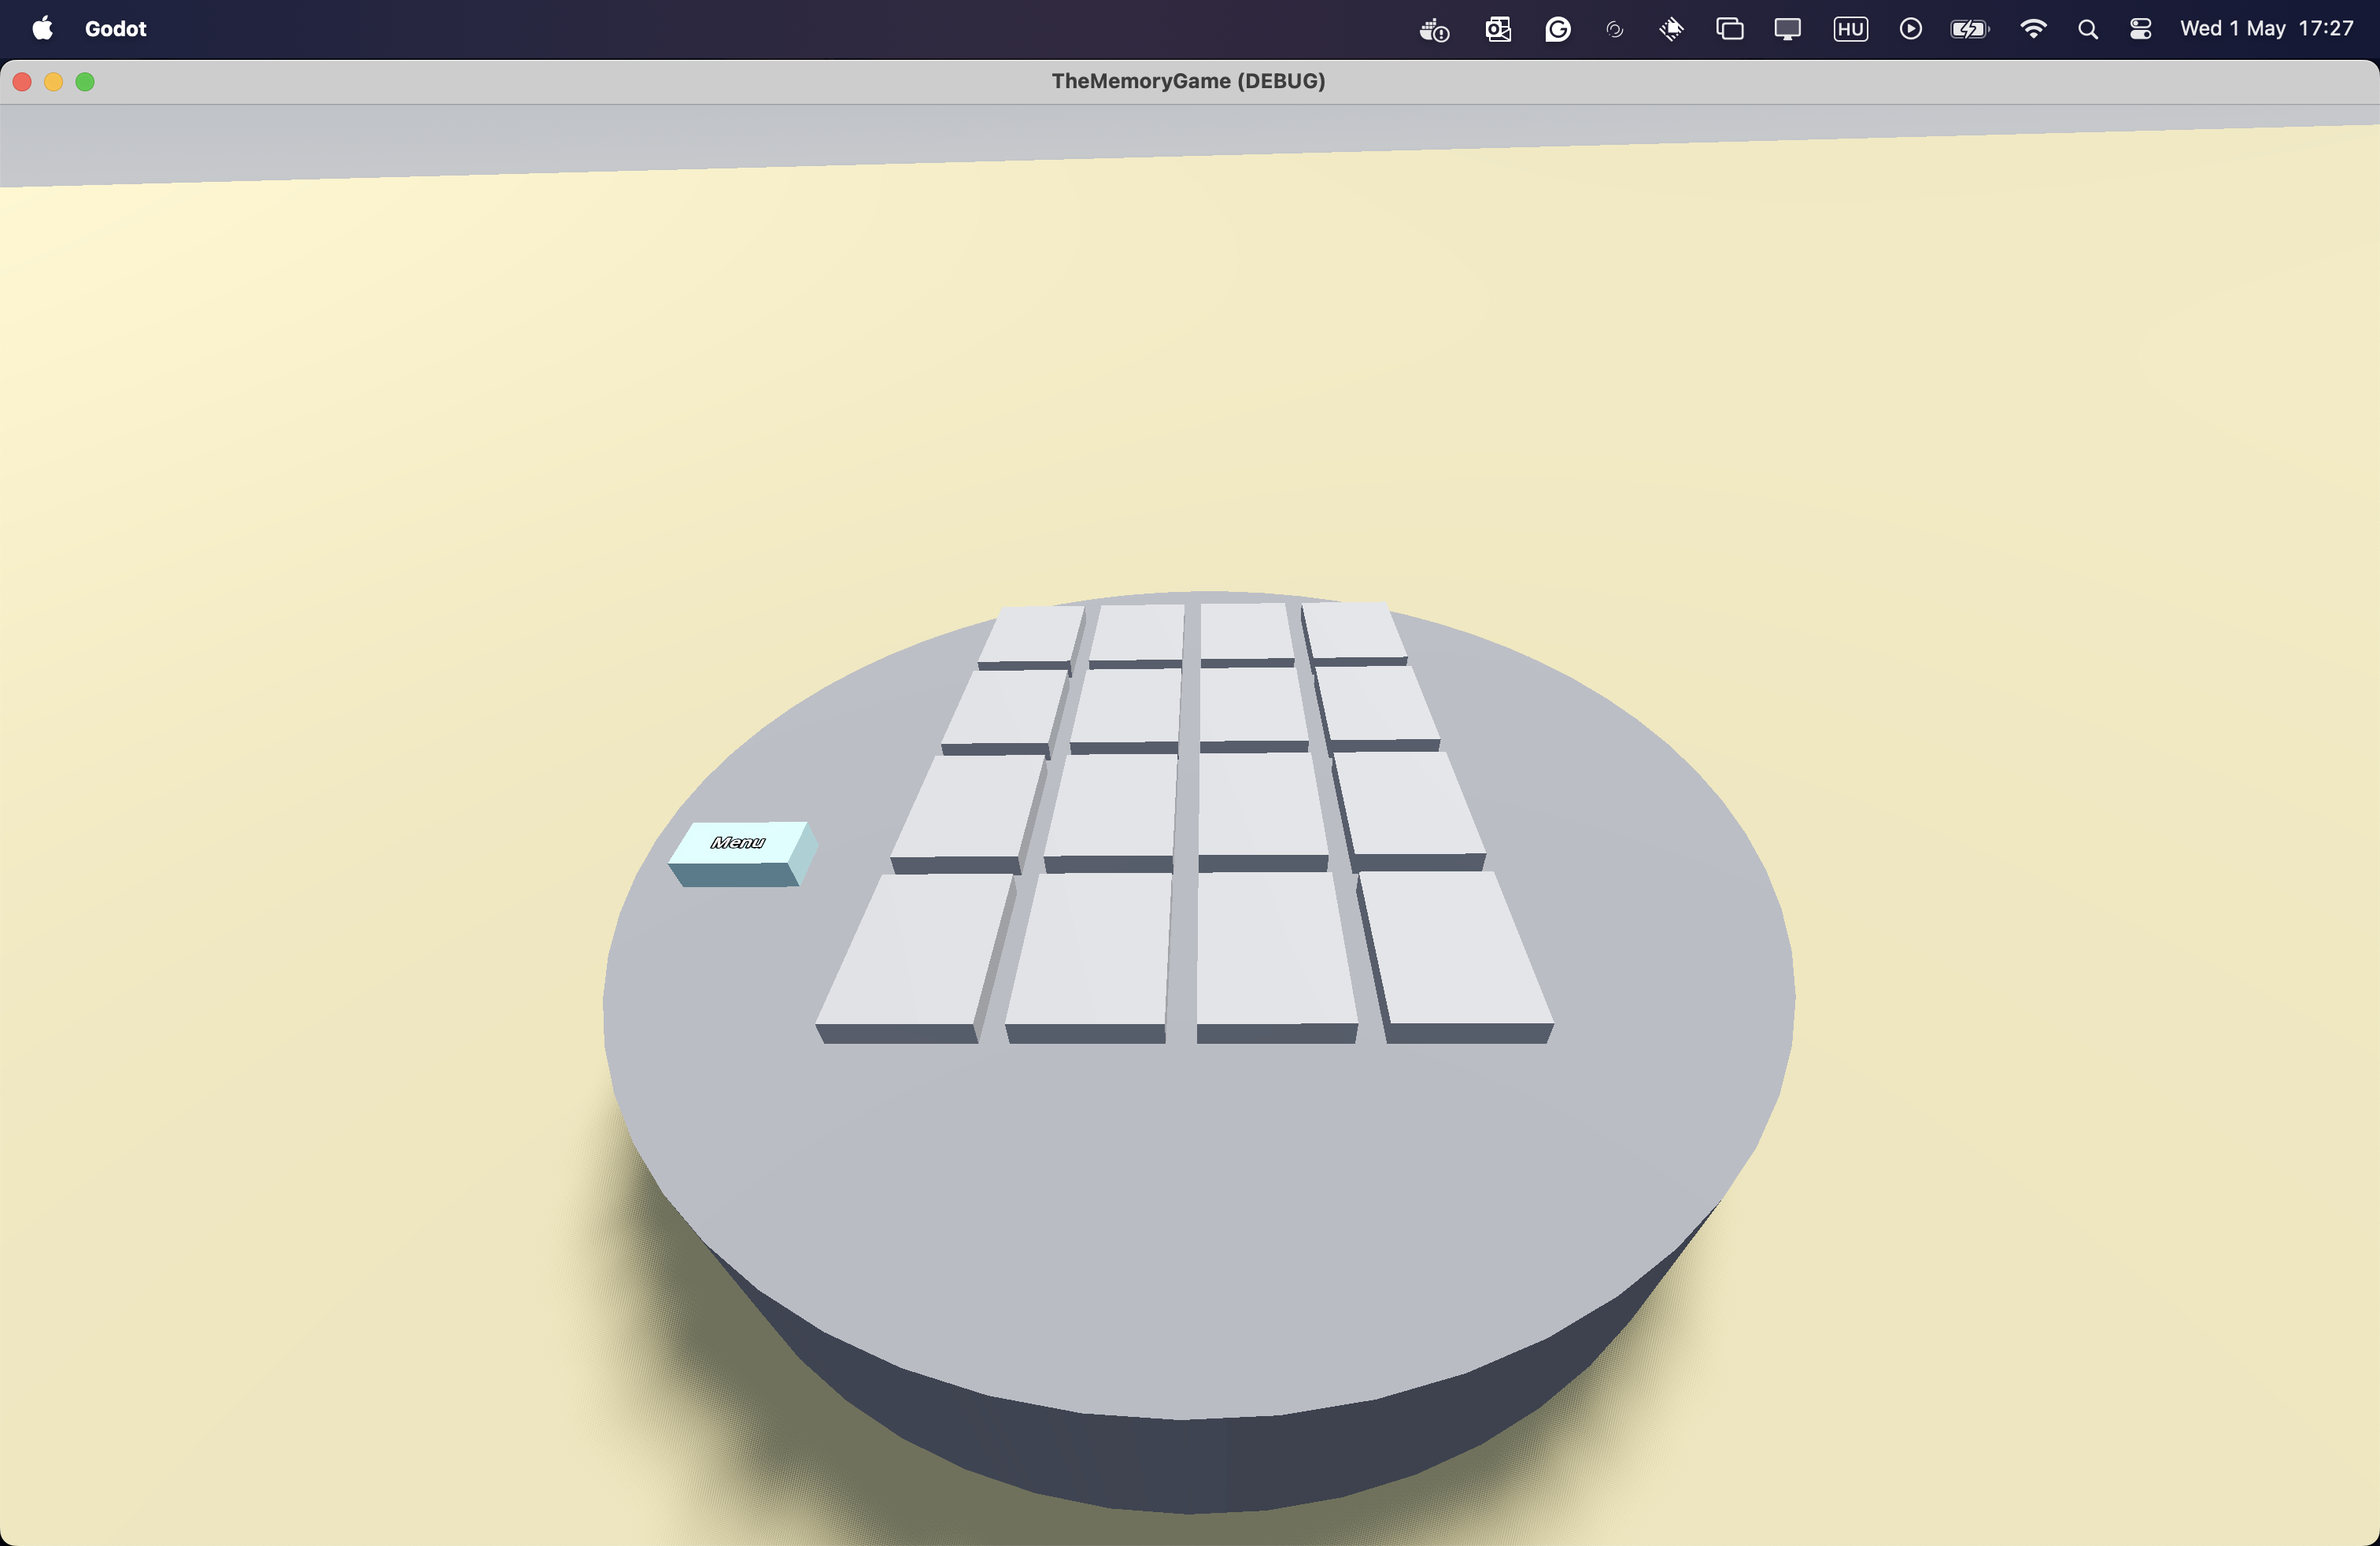
\includegraphics[width=\textwidth]{img/asztal_4x4.png}
    \caption{4x4-es memóriajáték kezdő állapota}
    \label{img:asztal}
\end{figure}
A kártyák előlapján betűk találhatók. Egyjátékos esetben a játékos célja, hogy minél kevesebb kártyapár megfordításából megtalálja az összes memória párt. Többjátékos esetben, hogy ő szerezze a legtöbb pontot, vagyis több kártyapárt fordítson fel, mint az ellenfelei.


Ahhoz, hogy egy kártyát megfordítson, a játékosnak rá kell kattintania. Ekkor láthatóvá válik, mely betűhöz tartozik a memória elemhez (\ref{img:kartya_fliped}. ábra). 
A megfordított kártyához választani kell egy másikat. A játékosnak törekednie kell, hogy korábbi ismeretei alapján, a következőre a választott kártya előlapján ugyanaz a betű szerepeljen, mint a már felfordított memória lapon, vagyis egy párt fordítson fel. 
Értelemszerűen ez az első felfordításkor nem lehetséges, hiszen nincs korábbi ismerete a játékról (\ref{img:non_pair}. ábra).
\begin{figure}[h]
\begin{subfigure}[t]{0.5\textwidth}
    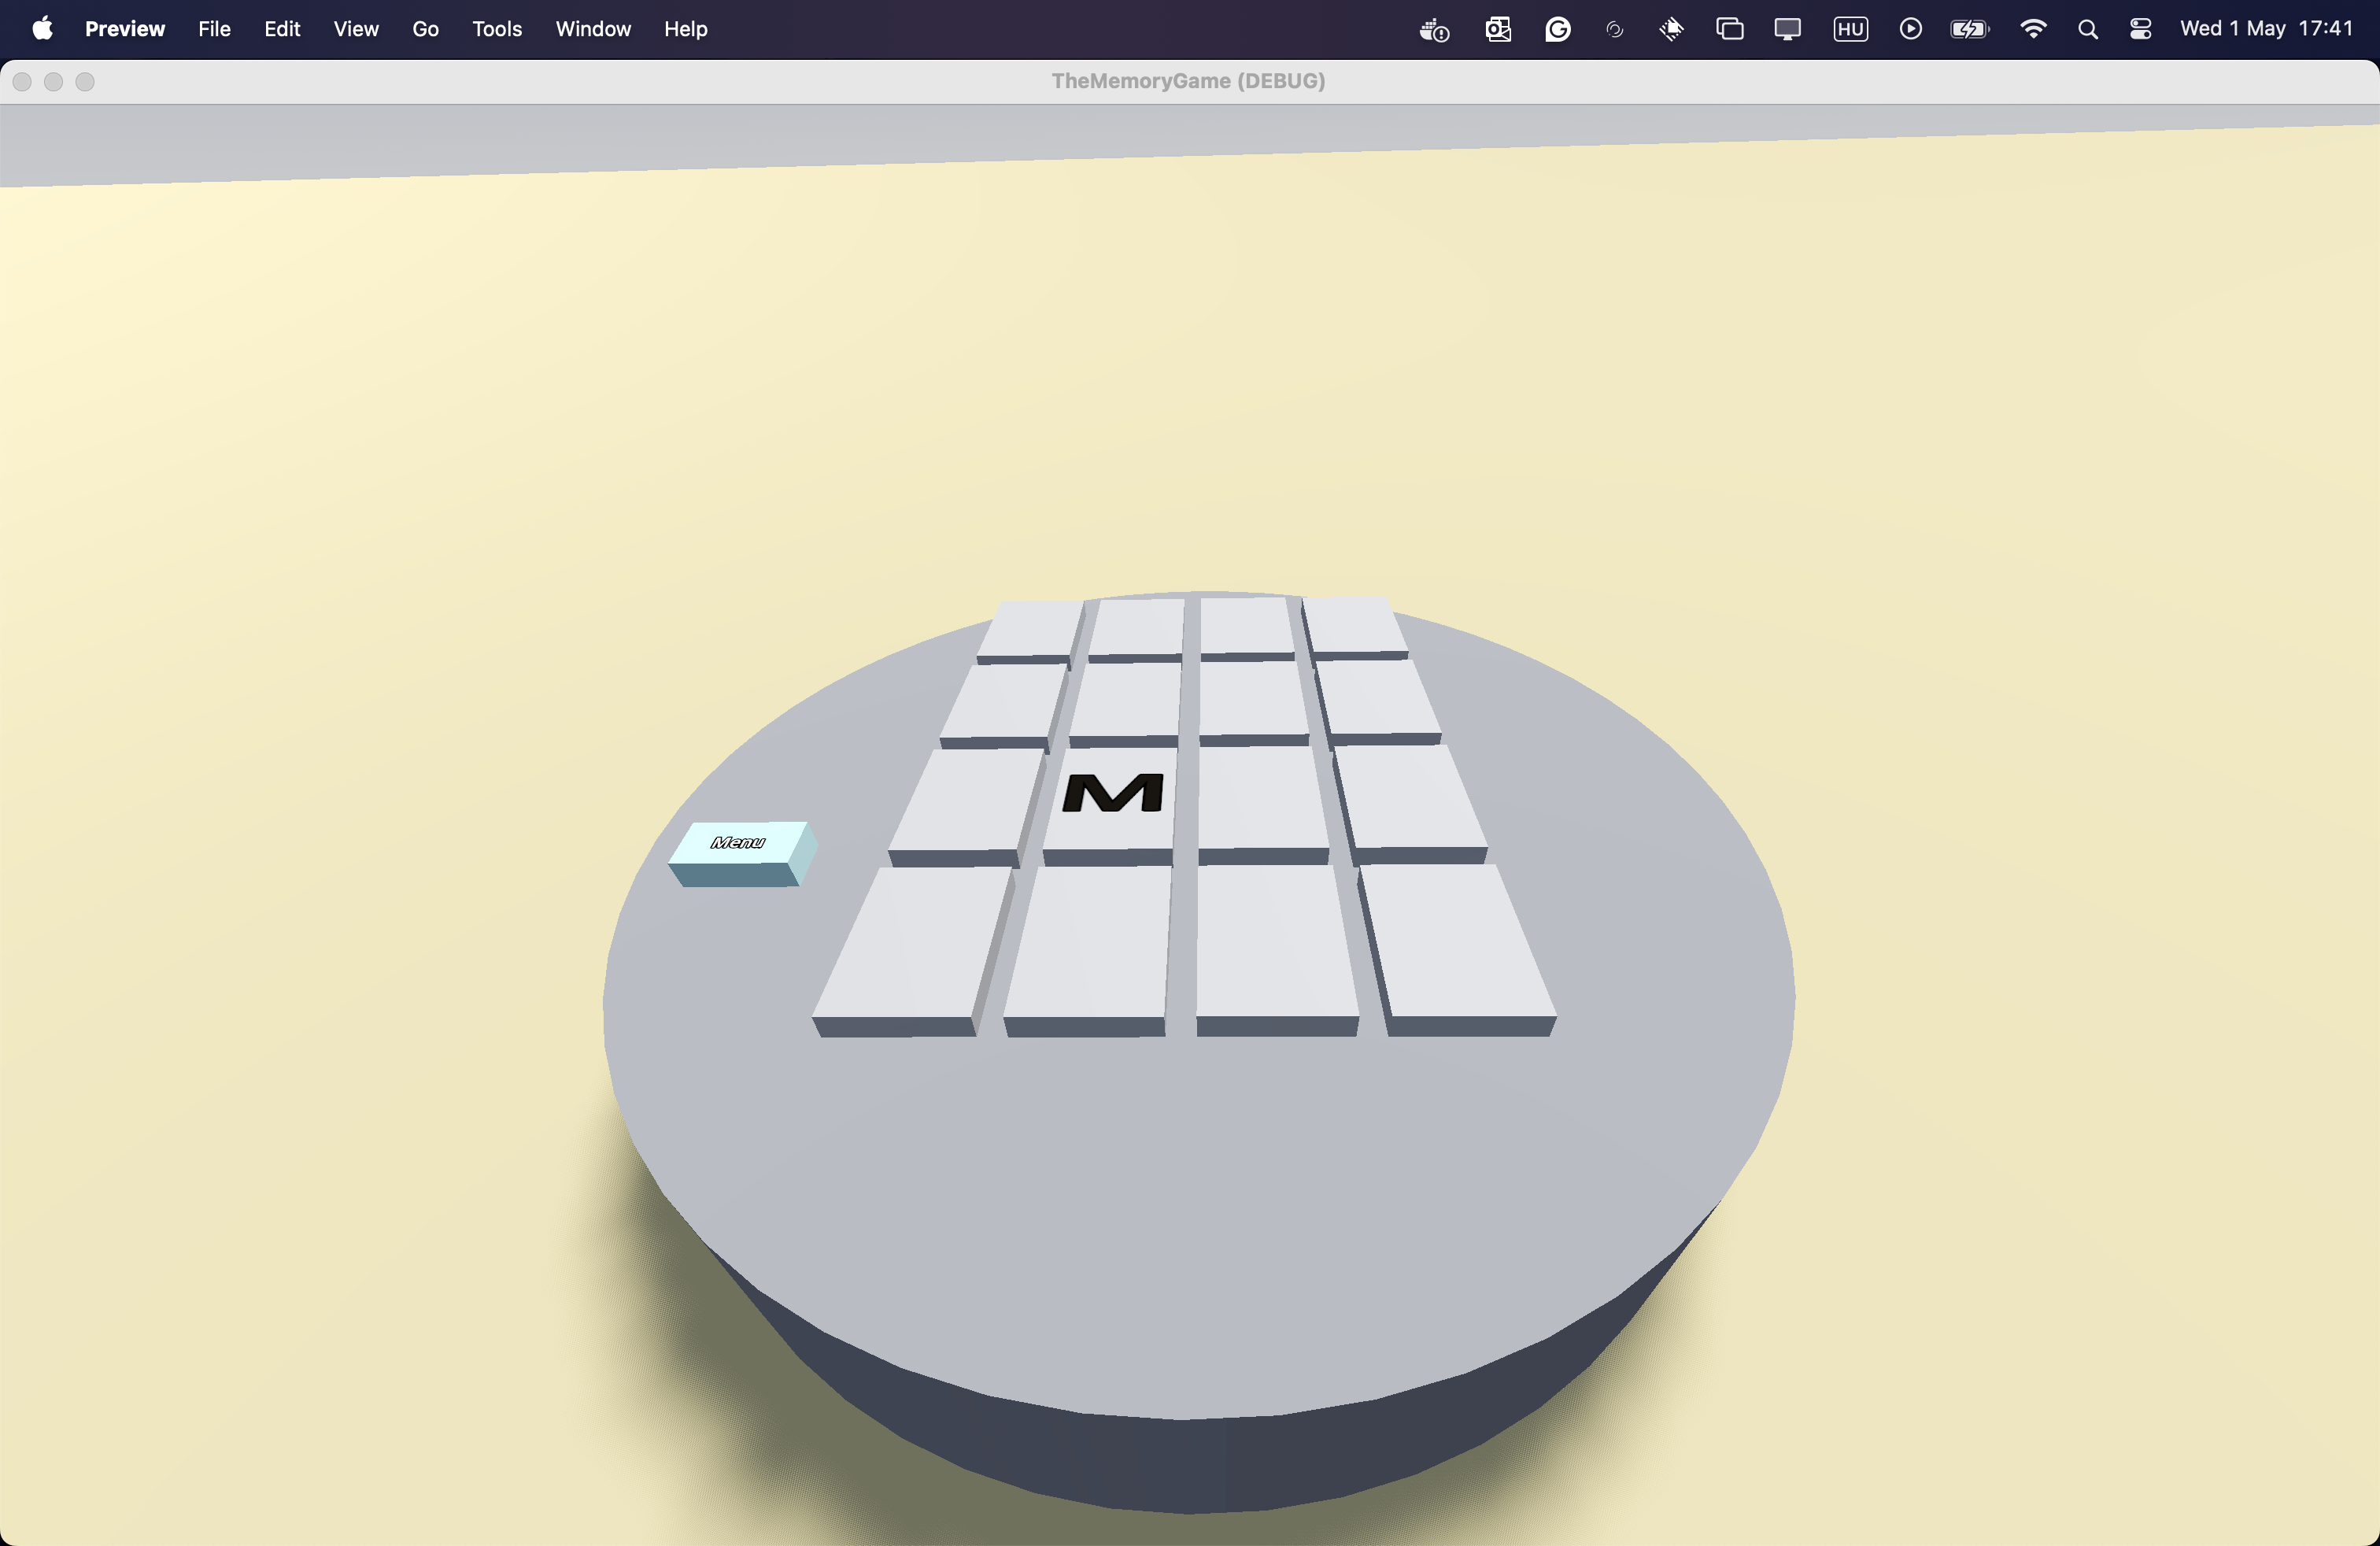
\includegraphics[width=\linewidth]{img/asztal_4x4_card_flipped.png}
    \caption{Egy kártya ki van választva}
    \label{img:kartya_fliped}
\end{subfigure}
\begin{subfigure}[t]{0.5\textwidth}
    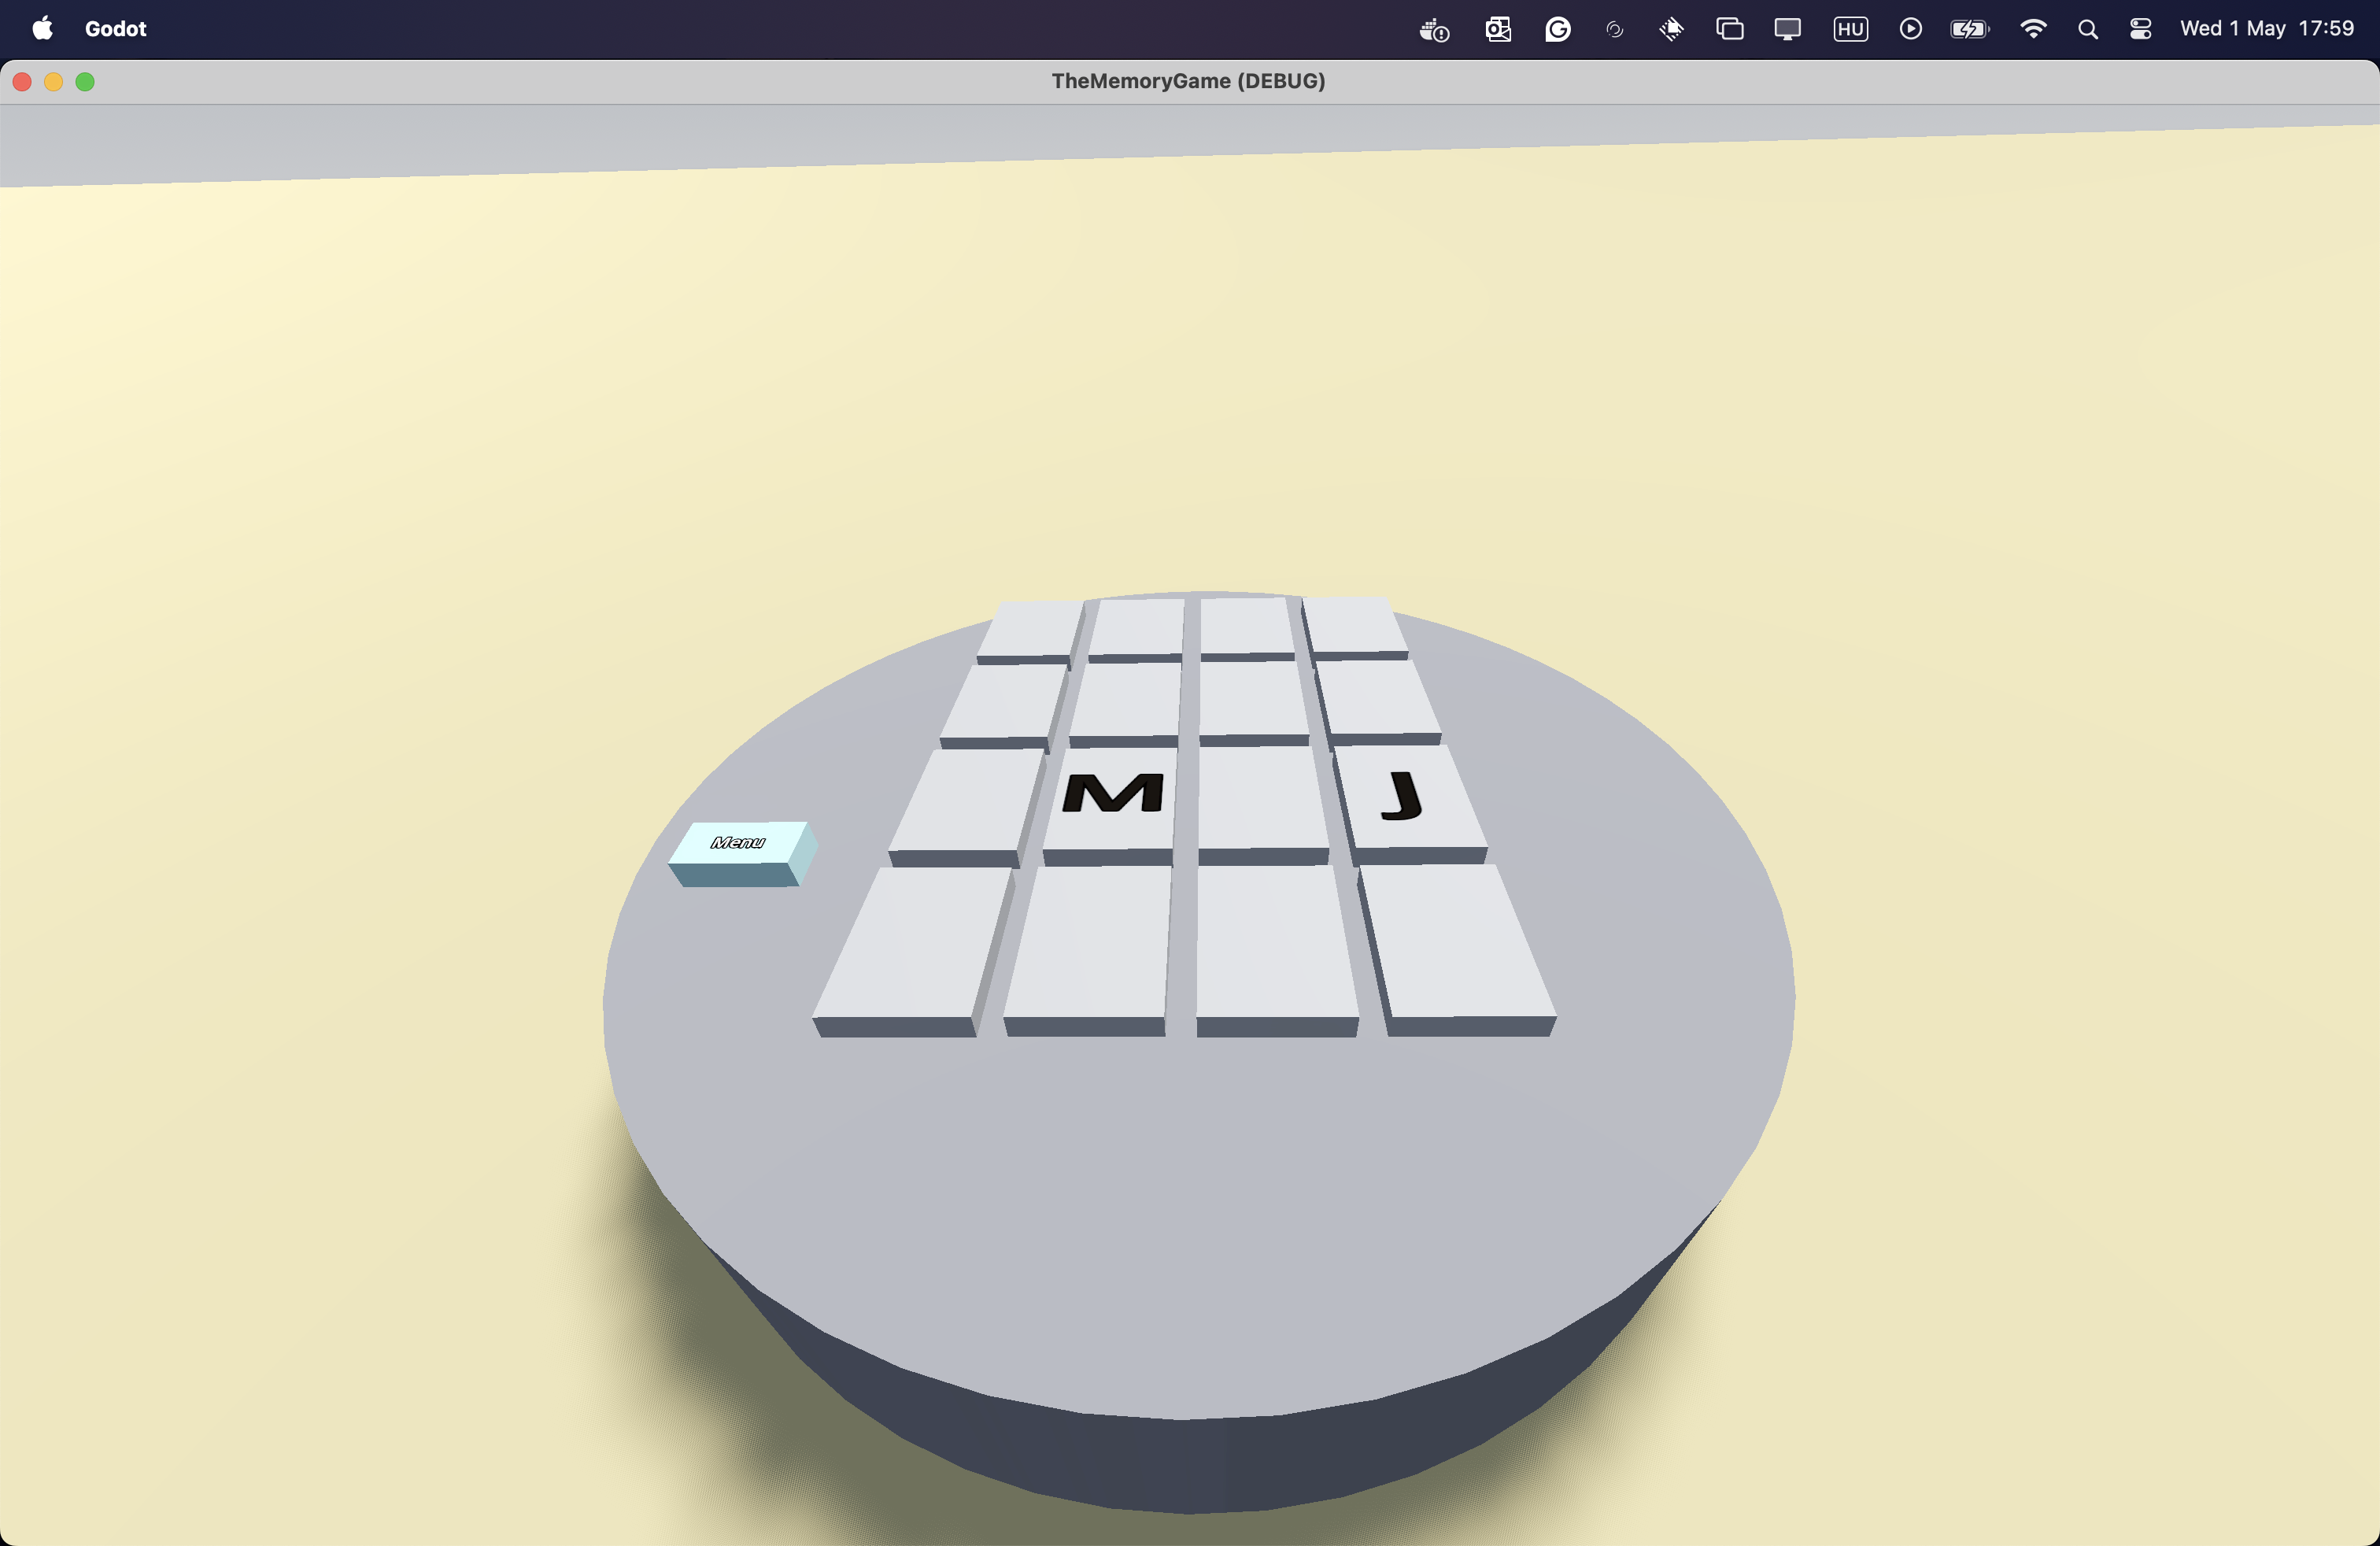
\includegraphics[width=\linewidth]{img/asztal_4x4_non_pair.png}
    \caption{Mivel a betűk nem azonosak, ezér ez nem egy pár, visszafordítjuk a kártyákat.}
    \label{img:non_pair}
\end{subfigure}
\caption{4x4-es játék, példa kör, amikor nem egy párt húzunk fel}
\end{figure}
Ha a felfordított kártyák nem alkotnak párt, akkor a kártyák maguktól visszafordulnak pár másodperc elteltével. Ez után egyszemélyes játék esetén esetén végrehajtunk egy újabb fordítást. Többjátékos esetén a következő játékos végezheti el a körét. 

Ha párt alkotnak (\ref{img:pair}. ábra), akkor a kártyák eltűnnek a játékmezőről  (\ref{img:pair_gone}. ábra).Többjátékos esetben a felfordított játékos kap egy pontot, és egy újabb fordítással folytatja a körét, mindaddig, míg egy nem párt fordít.
\begin{figure}[H]
    \begin{subfigure}[ct]{0.5\textwidth}
        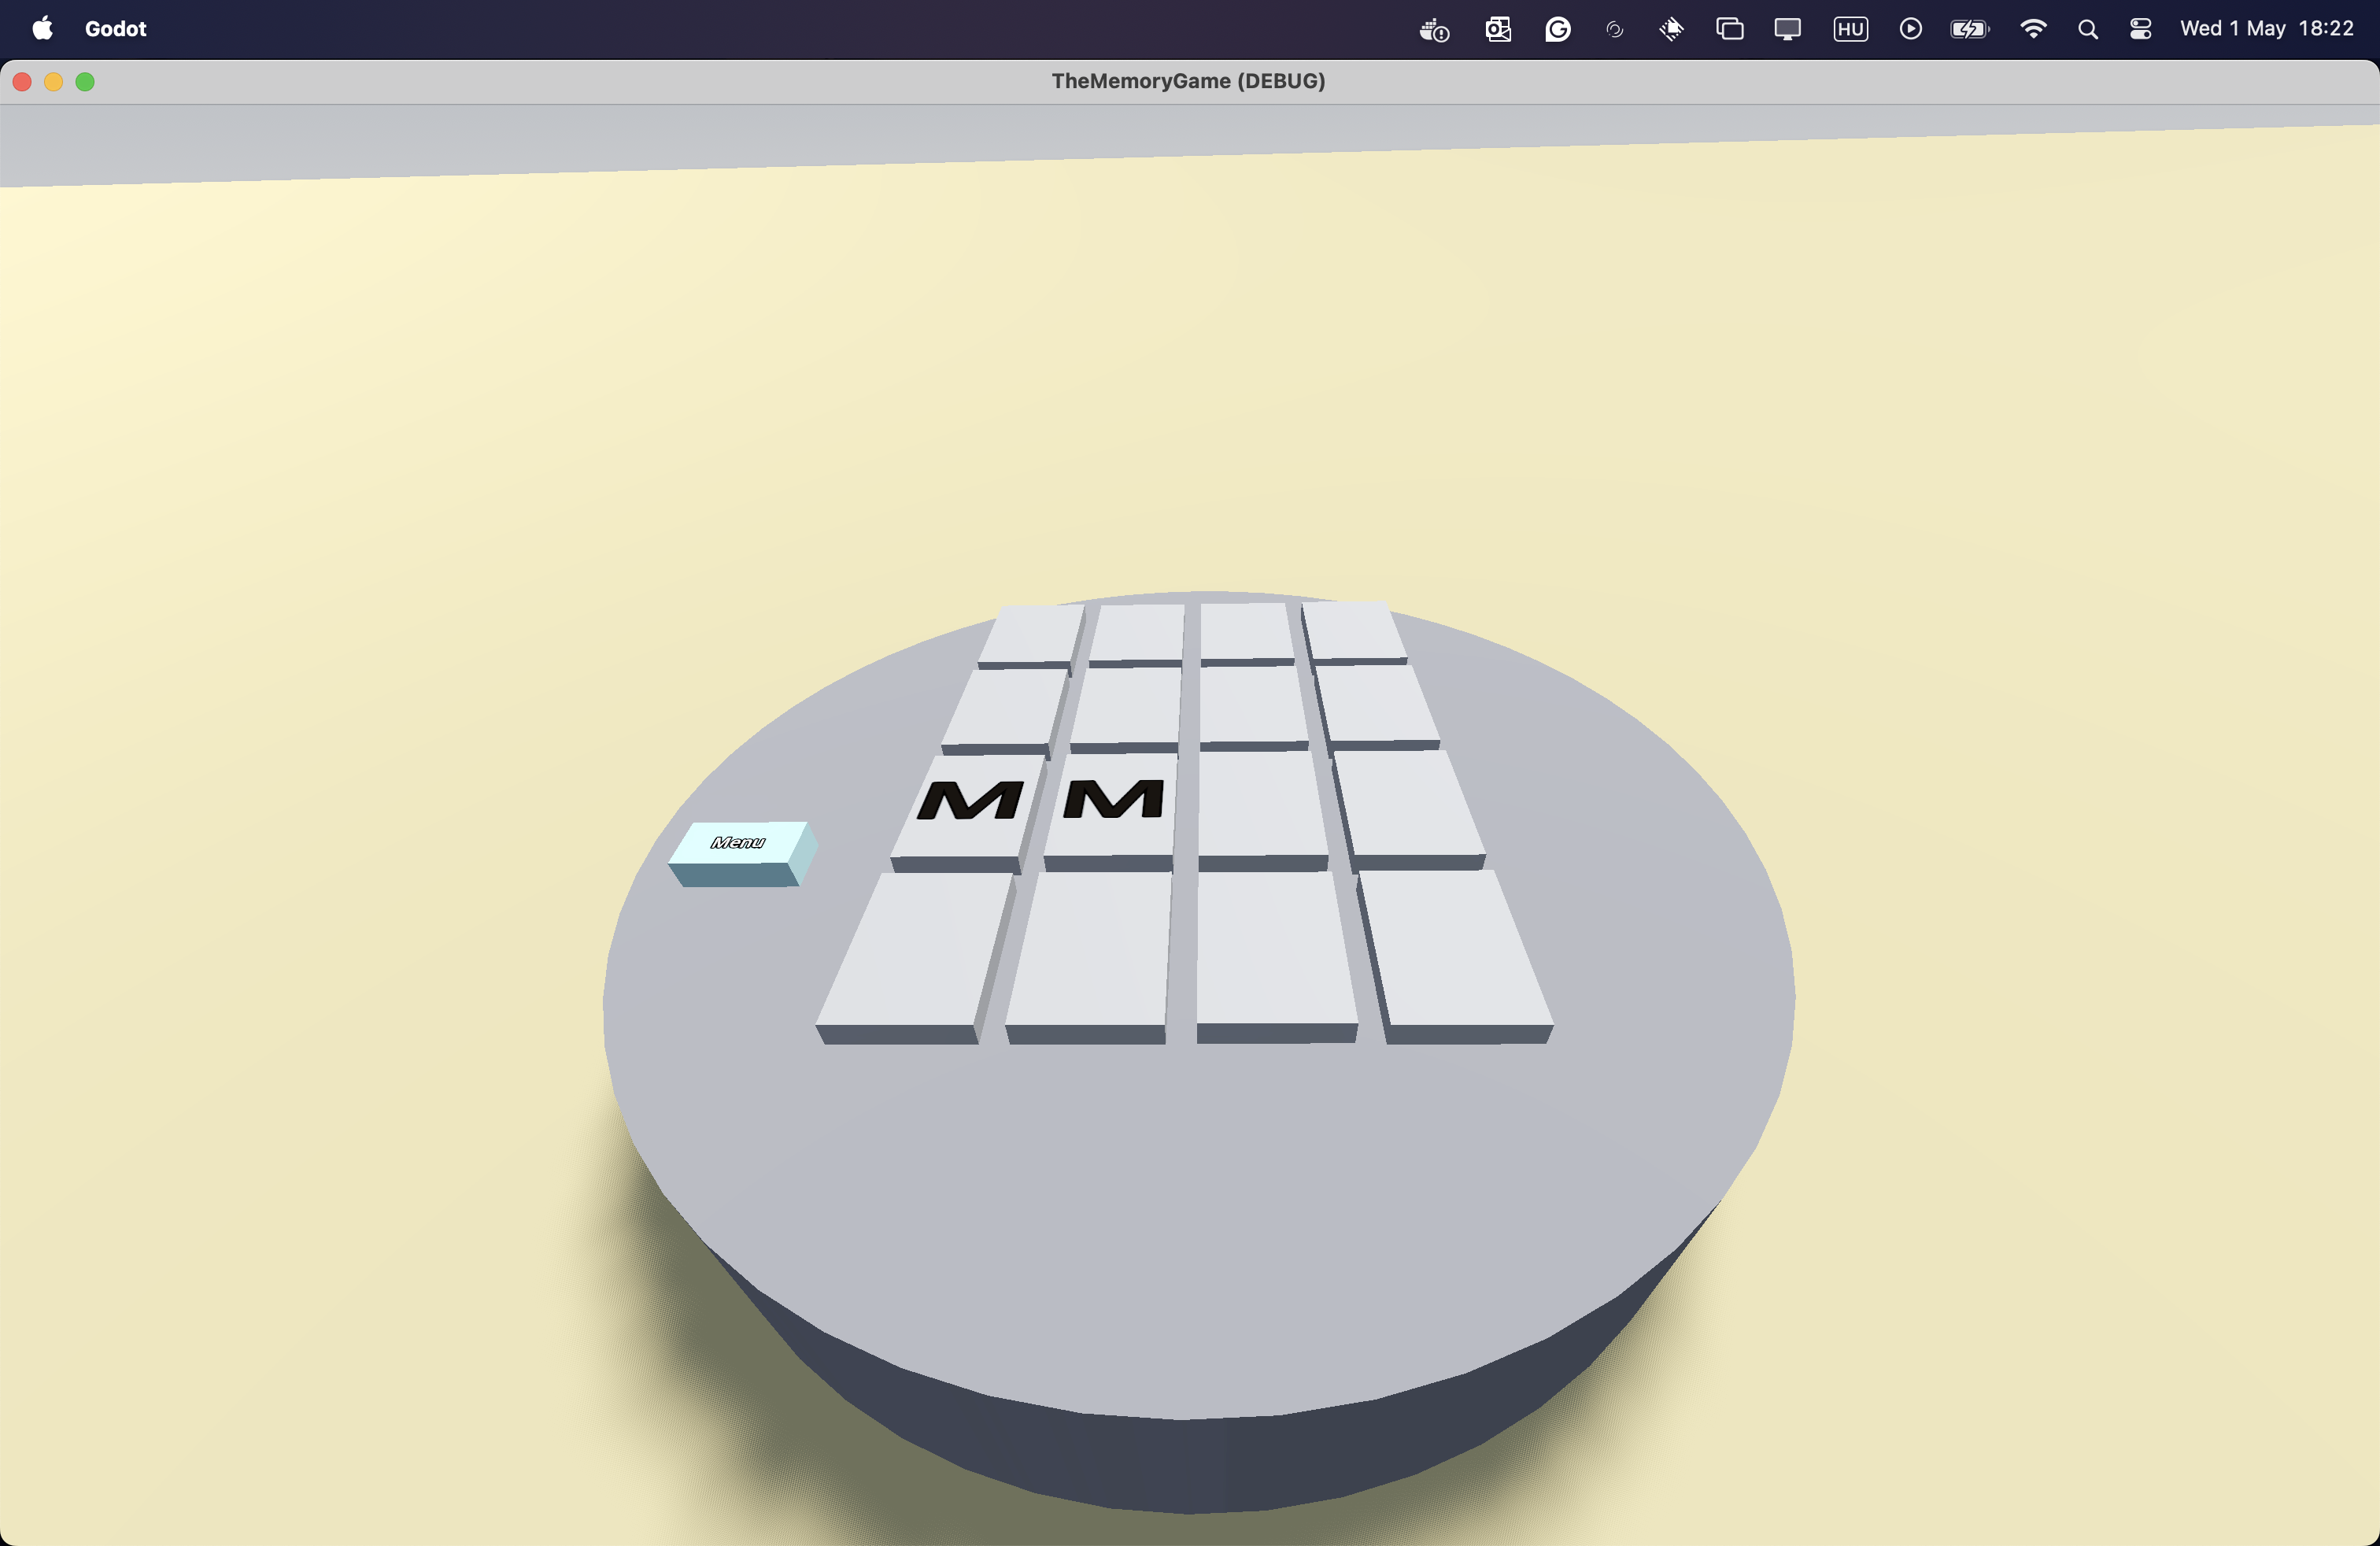
\includegraphics[width=\textwidth]{img/asztal_4x4_pair.png}
        \caption{A kiválasztott kártyák párt alkotnak}
        \label{img:pair}
    \end{subfigure}
    \begin{subfigure}[ct]{0.5\textwidth}
        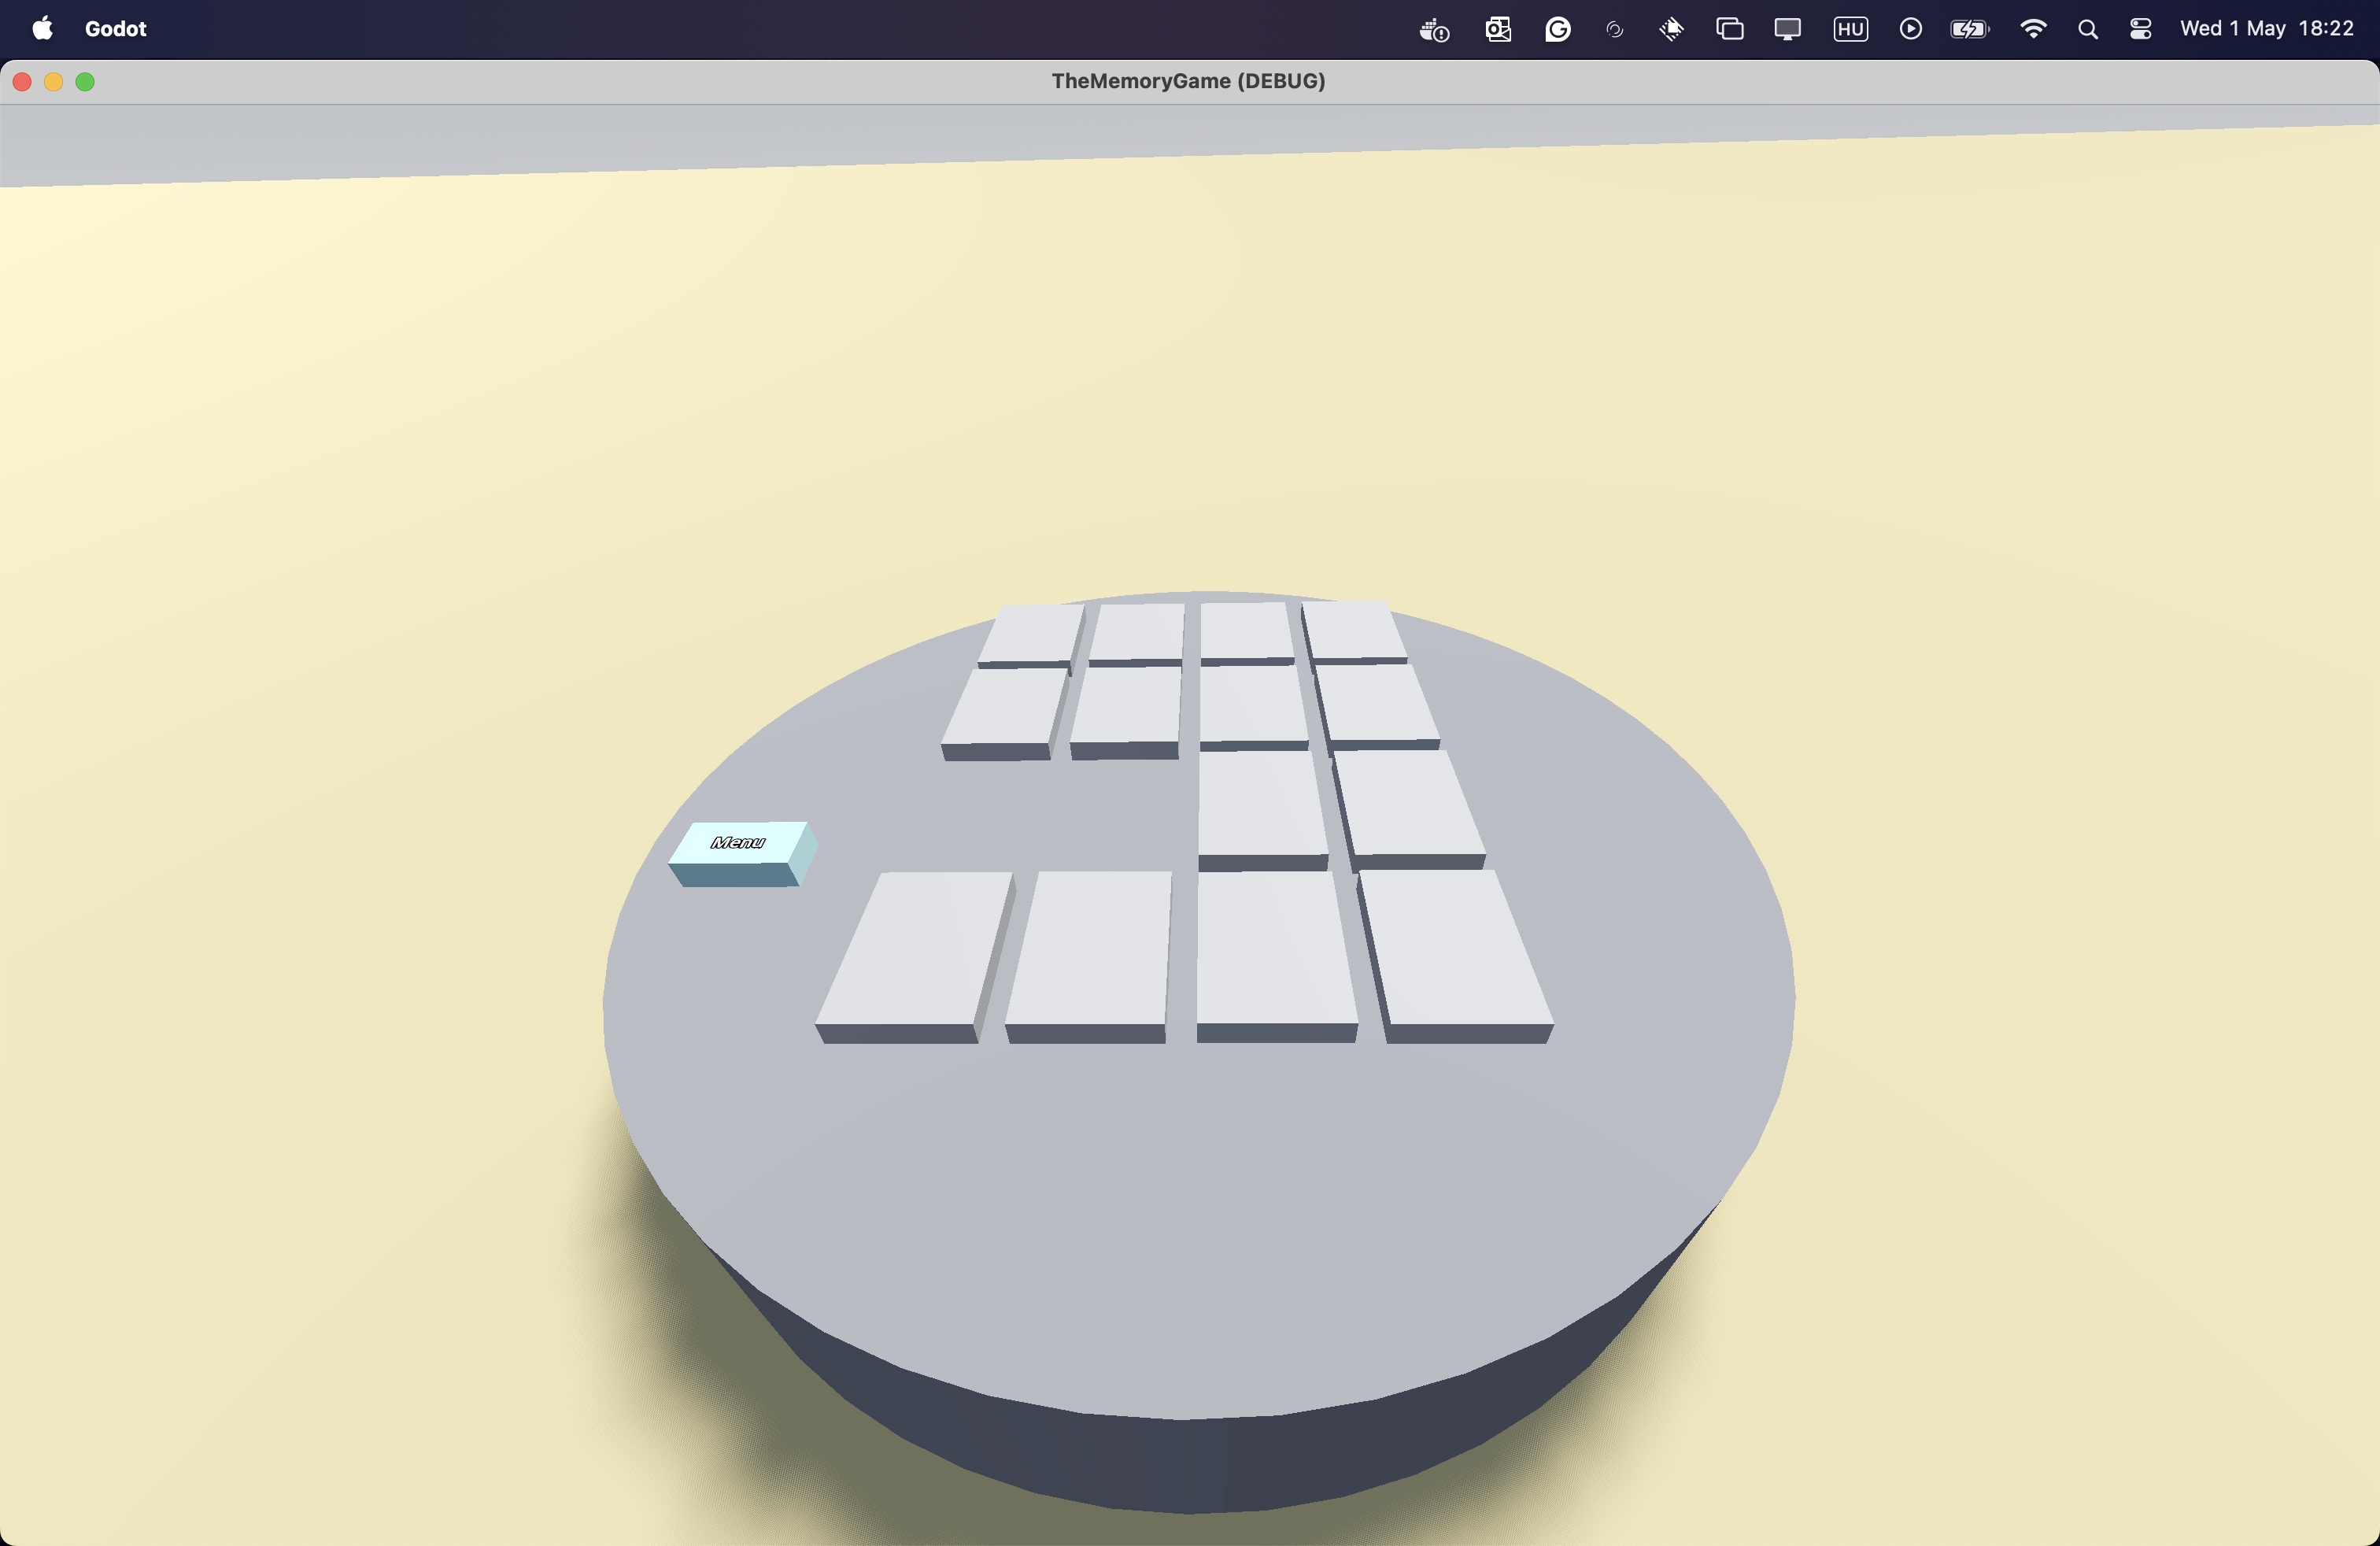
\includegraphics[width=\textwidth]{img/asztal_4x4_pair_eltunik.png}
        \caption{Eltűnik a pár az asztalról}
        \label{img:pair_gone}
    \end{subfigure}
    \caption{4x4-es játék, példa kör, amikor egy párt húzunk fel}
\end{figure}


Amint az összes kártya eltűnik az asztalról, a játék véget ér, és visszakerülünk a menübe.
A játékba több nehézségi szintet tettünk, melyet a menüből érhetünk el (\ref{img:menu}. ábra). A különböző menüpontok, a kártyák számának elhelyezkedését jelölik.
\begin{figure}[h]
    \centering
    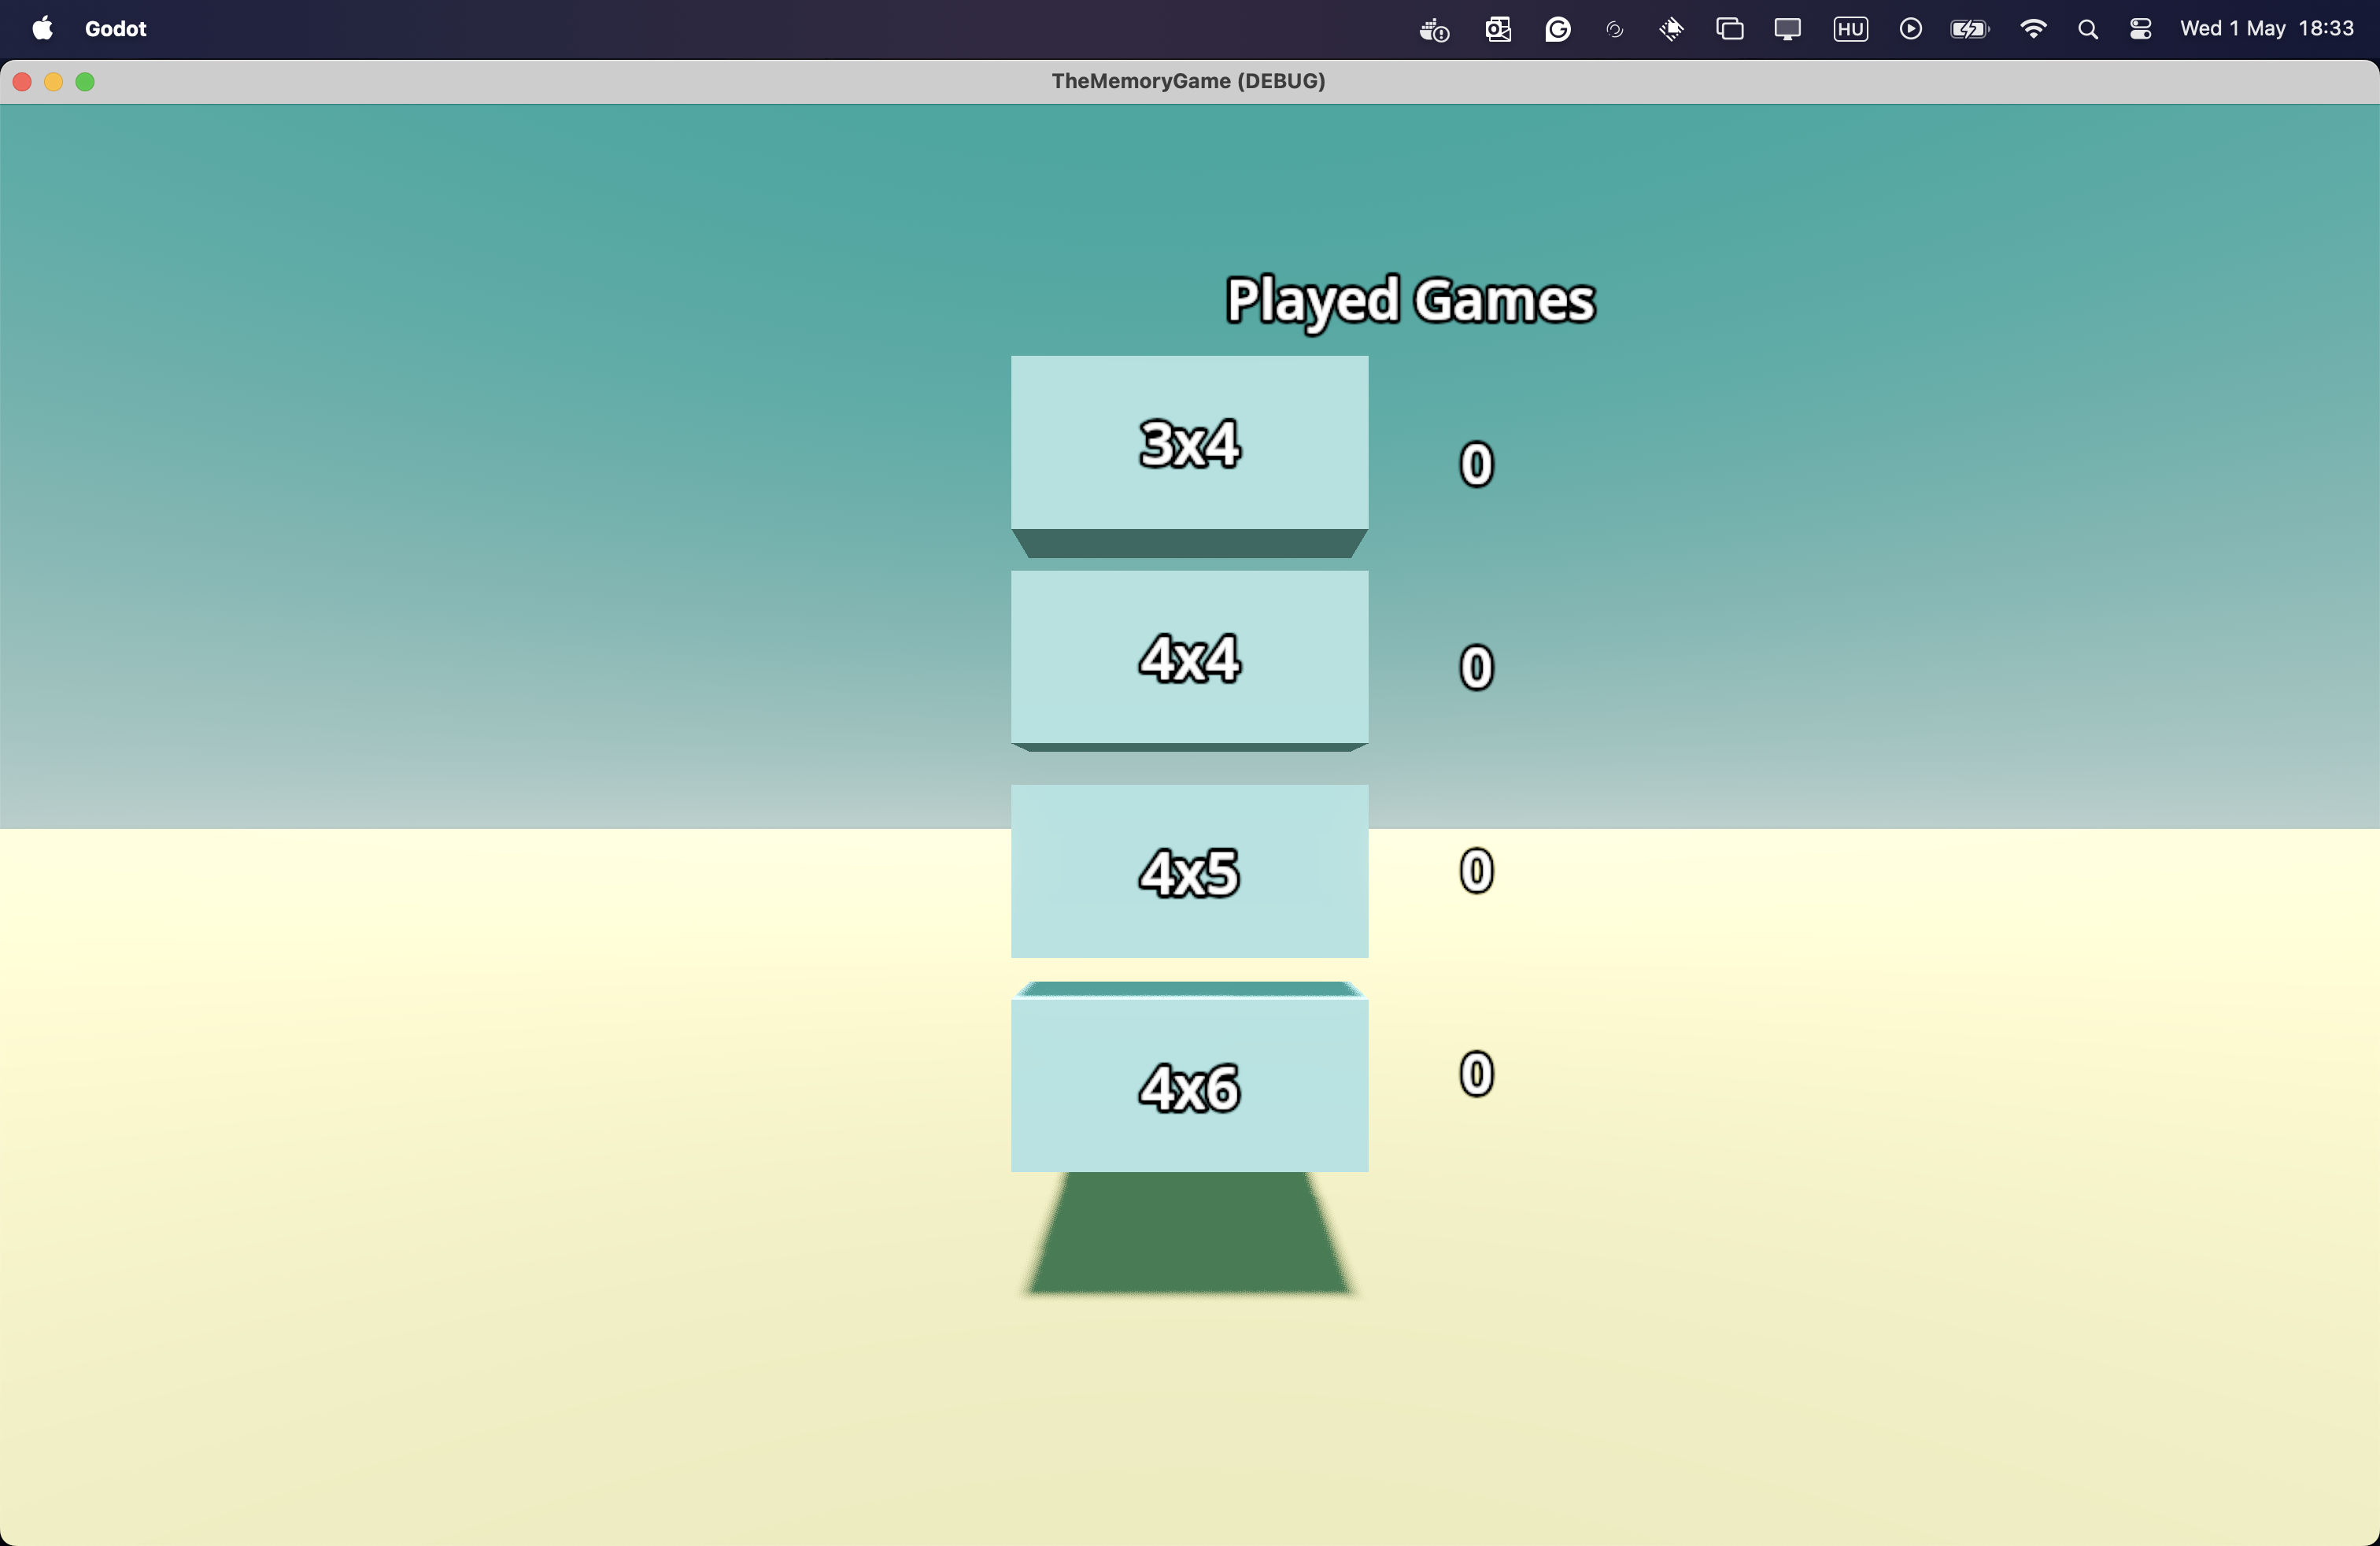
\includegraphics[width=0.5\textwidth]{img/menu.png}
    \caption{A játék menüje}
    \label{img:menu}  
\end{figure}

\section{Struktúrális felépítés}
A memória játék a Godot elveinek megfelelően Node-okból és Scene-ekből \cite{godotengineNodesScenes} áll. A Scene-ek struktúrája a következő.
\subsection{Menü}


A Játék menüje (\ref{img:menu_scene}. ábra), a következő módon épül fel. A Gombok olyan MeshInstance3D Node-ok \cite{godotengineMeshInstance3D}, melyekre ha a játékos rákattint, akkor emittálnak egy \lstinline{button_pressed()} signal-t (\ref{code:button_pressed_signal}. ábra).
A MenuScene kódjában hallgatózunk erre külön külön a gombokra. A megfelelő gomb megnyomásával beállítjuk a \lstinline{Constant.CARD_PAIR_NUMBER} globális változót, mely segítségével létrehozzuk a \lstinline{basic_scene}-t.
\begin{figure}[h]
    \centering
    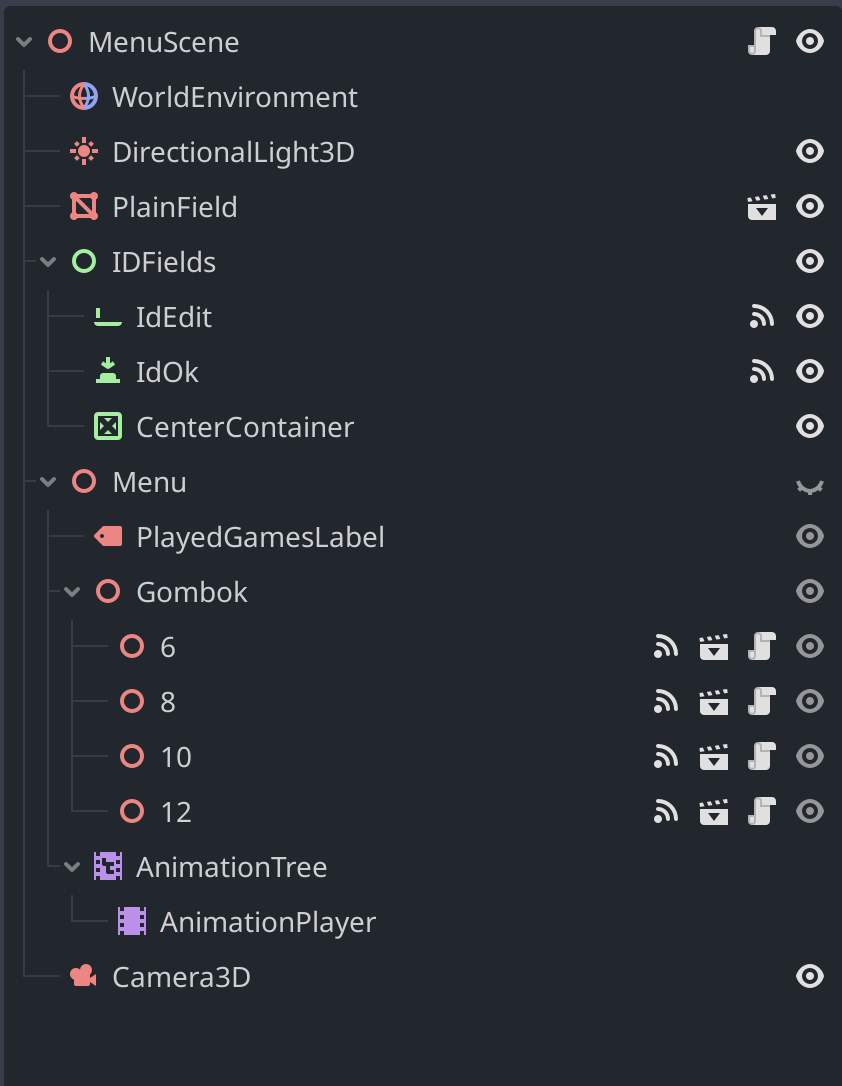
\includegraphics[width=0.5\textwidth]{img/menu_scene_tree.png}
    \caption{A játék menü Scene-jének struktúrája}
    \label{img:menu_scene}  
\end{figure}

\begin{figure}[H]
    \centering
    \begin{lstlisting}[language=GDScript]
    func _on_area_3d_input_event(camera, event, position, normal, shape_idx):
        if event is InputEventMouseButton:
            if (event.button_index == MOUSE_BUTTON_LEFT && event.pressed == true):
                emit_signal("button_pressed")
    
    func set_number_label_text(new_label_text: String):
        number_label.text = new_label_text;
    \end{lstlisting}
    \caption{A menü gombja  \lstinline{button_pressed} signal-t emittál}
    \label{code:button_pressed_signal}
\end{figure}

\subsection{Basic Scene}

A Basic Scene (\ref{img:basic_scene}. ábra) struktúrája dinamikusan épül fel a \lstinline{Card} Scene-ekből, melyet a \lstinline|Deck| globális objektum ad oda a \lstinline|Basic Scene| -nek. 
\begin{figure}[H]
    \centering
    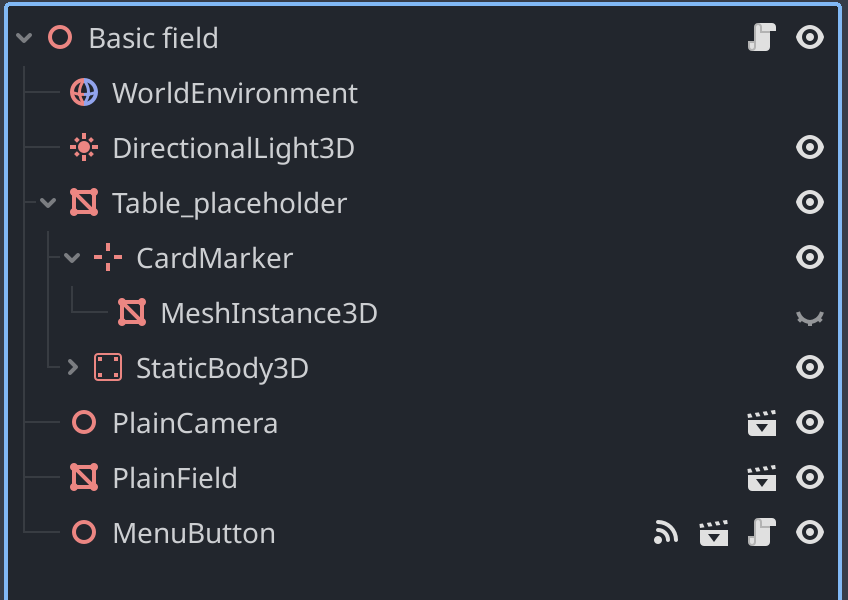
\includegraphics[width=0.5\textwidth]{img/basic_field_scene_structure.png}
    \caption{A játéktér Scene struktúrális felépítése}
    \label{img:basic_scene}  
\end{figure}
A scene kiszámolja, az előre beállított kártya szélesség, magasság és margó konstansok alapján, hogy a megkapott kártyák számát, a \lstinline|CardMarker| -höz képest hova kell lerakni (\ref{code:calculate_coordinate}. ábra)
\begin{figure}[H]
    \centering
    \begin{lstlisting}[language=GDScript]
        func _calculate_coordinate(i, j):
        return Vector3(
            TABLE.position.x + (((CARD_WIDTH  + MARGO) * CARD_SCALE) * i ) - (((CARD_WIDTH * CARD_ROW) - (CARD_WIDTH) + (MARGO*(CARD_ROW-1)))*CARD_SCALE / 2),
            TABLE.position.y,
            TABLE.position.z + (((CARD_HEIGHT  + MARGO) * CARD_SCALE) * j ) - (((CARD_HEIGHT * CARD_COLUMN) - (CARD_HEIGHT) + (MARGO*(CARD_COLUMN-1)))*CARD_SCALE / 2)
        )
    \end{lstlisting}
    \caption{Kártyák koordinátájának kiszámítása}
    \label{code:calculate_coordinate}
\end{figure}
Amint a \lstinline|Deck| objektum elküldi a \lstinline{cards_empty} signal-t, vagyis a játék végét, vagy ha a játékos megnyomja a Menü gombot, a játék visszatér a menübe. 

Más feladata nincs. 


\subsection{Deck}
A \lstinline|Deck| egy olyan globális objektum, mely a program futása során bármikor elérhető. A feladatai: 
\begin{enumerate}
\item Létrehozni a kártyákat, a játék kezdetekor (\ref{code:make_deck}. ábra)
\item Folyamatosan figyeli, hogy mely \lstinline|Card|-ok vannak még játékban a lstinline|cards| tömbben.
\item Kezeli a kártyák felfordítását. Ha két kártya azonos, akkor azokat kiveszi a listájából (\ref{code:talalat}. ábra).
\item Lementeni a játékos minden lépését a data tömbbe a memóriába. 
\item Figyeli a játék végét.
\item Lementeni a data tömböt egy JSON file-ba a játék végével.
\end{enumerate}

\begin{figure}[h]
    \centering
    \begin{lstlisting}[language=GDScript]
    func make_deck(card_pair_number: int, card_scene: PackedScene):
        data.card_pair_number = card_pair_number;
        cards.clear();
        for i in range(0, card_pair_number):
            var word = "";
            while ABC.find(word) > - 1 or word == "":
                word = generate_word('abcdefghijklmnopqrst', 1).to_upper();
            ABC.push_back(word);
            var card = card_scene.instantiate();
            #call_deferred("add_child", card);
            if card.has_method("set_label"):
                card.set_label(word);
            cards.push_back(card);
            cards.push_back(card.duplicate());
        cards.shuffle();
        data.card_labels = ABC;
    \end{lstlisting}
    \caption{Létrehozzuk a kártyákat}
    \label{code:make_deck}
\end{figure}
\begin{figure}[h]
    \centering
    \begin{lstlisting}[language=GDScript]
func talalat():
	if (chosenA.get_label() == chosenB.get_label()):
		cards.remove_at(cards.find(chosenA));
		cards.remove_at(cards.find(chosenB));
		chosenA.queue_free();
		chosenB.queue_free();
	else:
		chosenA.play_card_reflip_animation();
		chosenB.play_card_reflip_animation();
	chosenA = null;
	chosenB = null;
	can_flip = true;
	if cards.size() == 0 :
		cards_empty.emit()
		save_data()
    \end{lstlisting}
    \caption{Figyeljük a találatot}
    \label{code:talalat}
\end{figure}


\subsection{Card}
A kartyak vagyis Card scene (\ref{img:card_tree}. ábra) rendelkezik egy \lstinline|labellel| amelyet a \lstinline|Deck| add neki, a kártya létrehozásakor. Ez mondja meg, hogy milyen kártya. 
Egy játékmezőn pontosan két egyforma labellel rendelkező kártya szerepel(\ref{img:cards_has_pairs}. ábra).

\begin{figure}[H]
    \centering
    \begin{minipage}[b]{0.45\textwidth}
        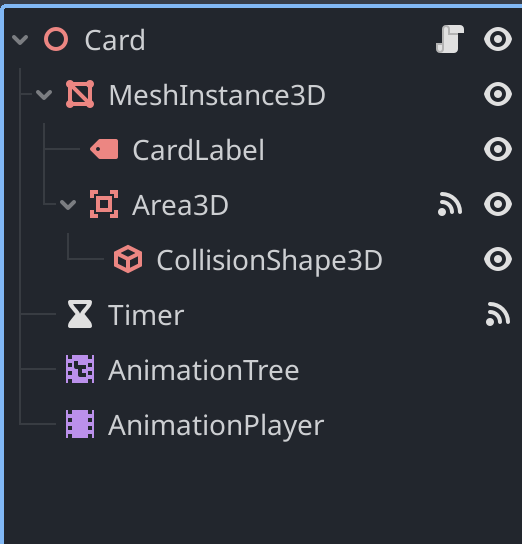
\includegraphics[width=\textwidth]{img/cards_scene_tree.png}
        \caption{A Card Scene struktúrája}
        \label{img:card_tree}
    \end{minipage}
    \hfill
    \begin{minipage}[b]{0.45\textwidth}
        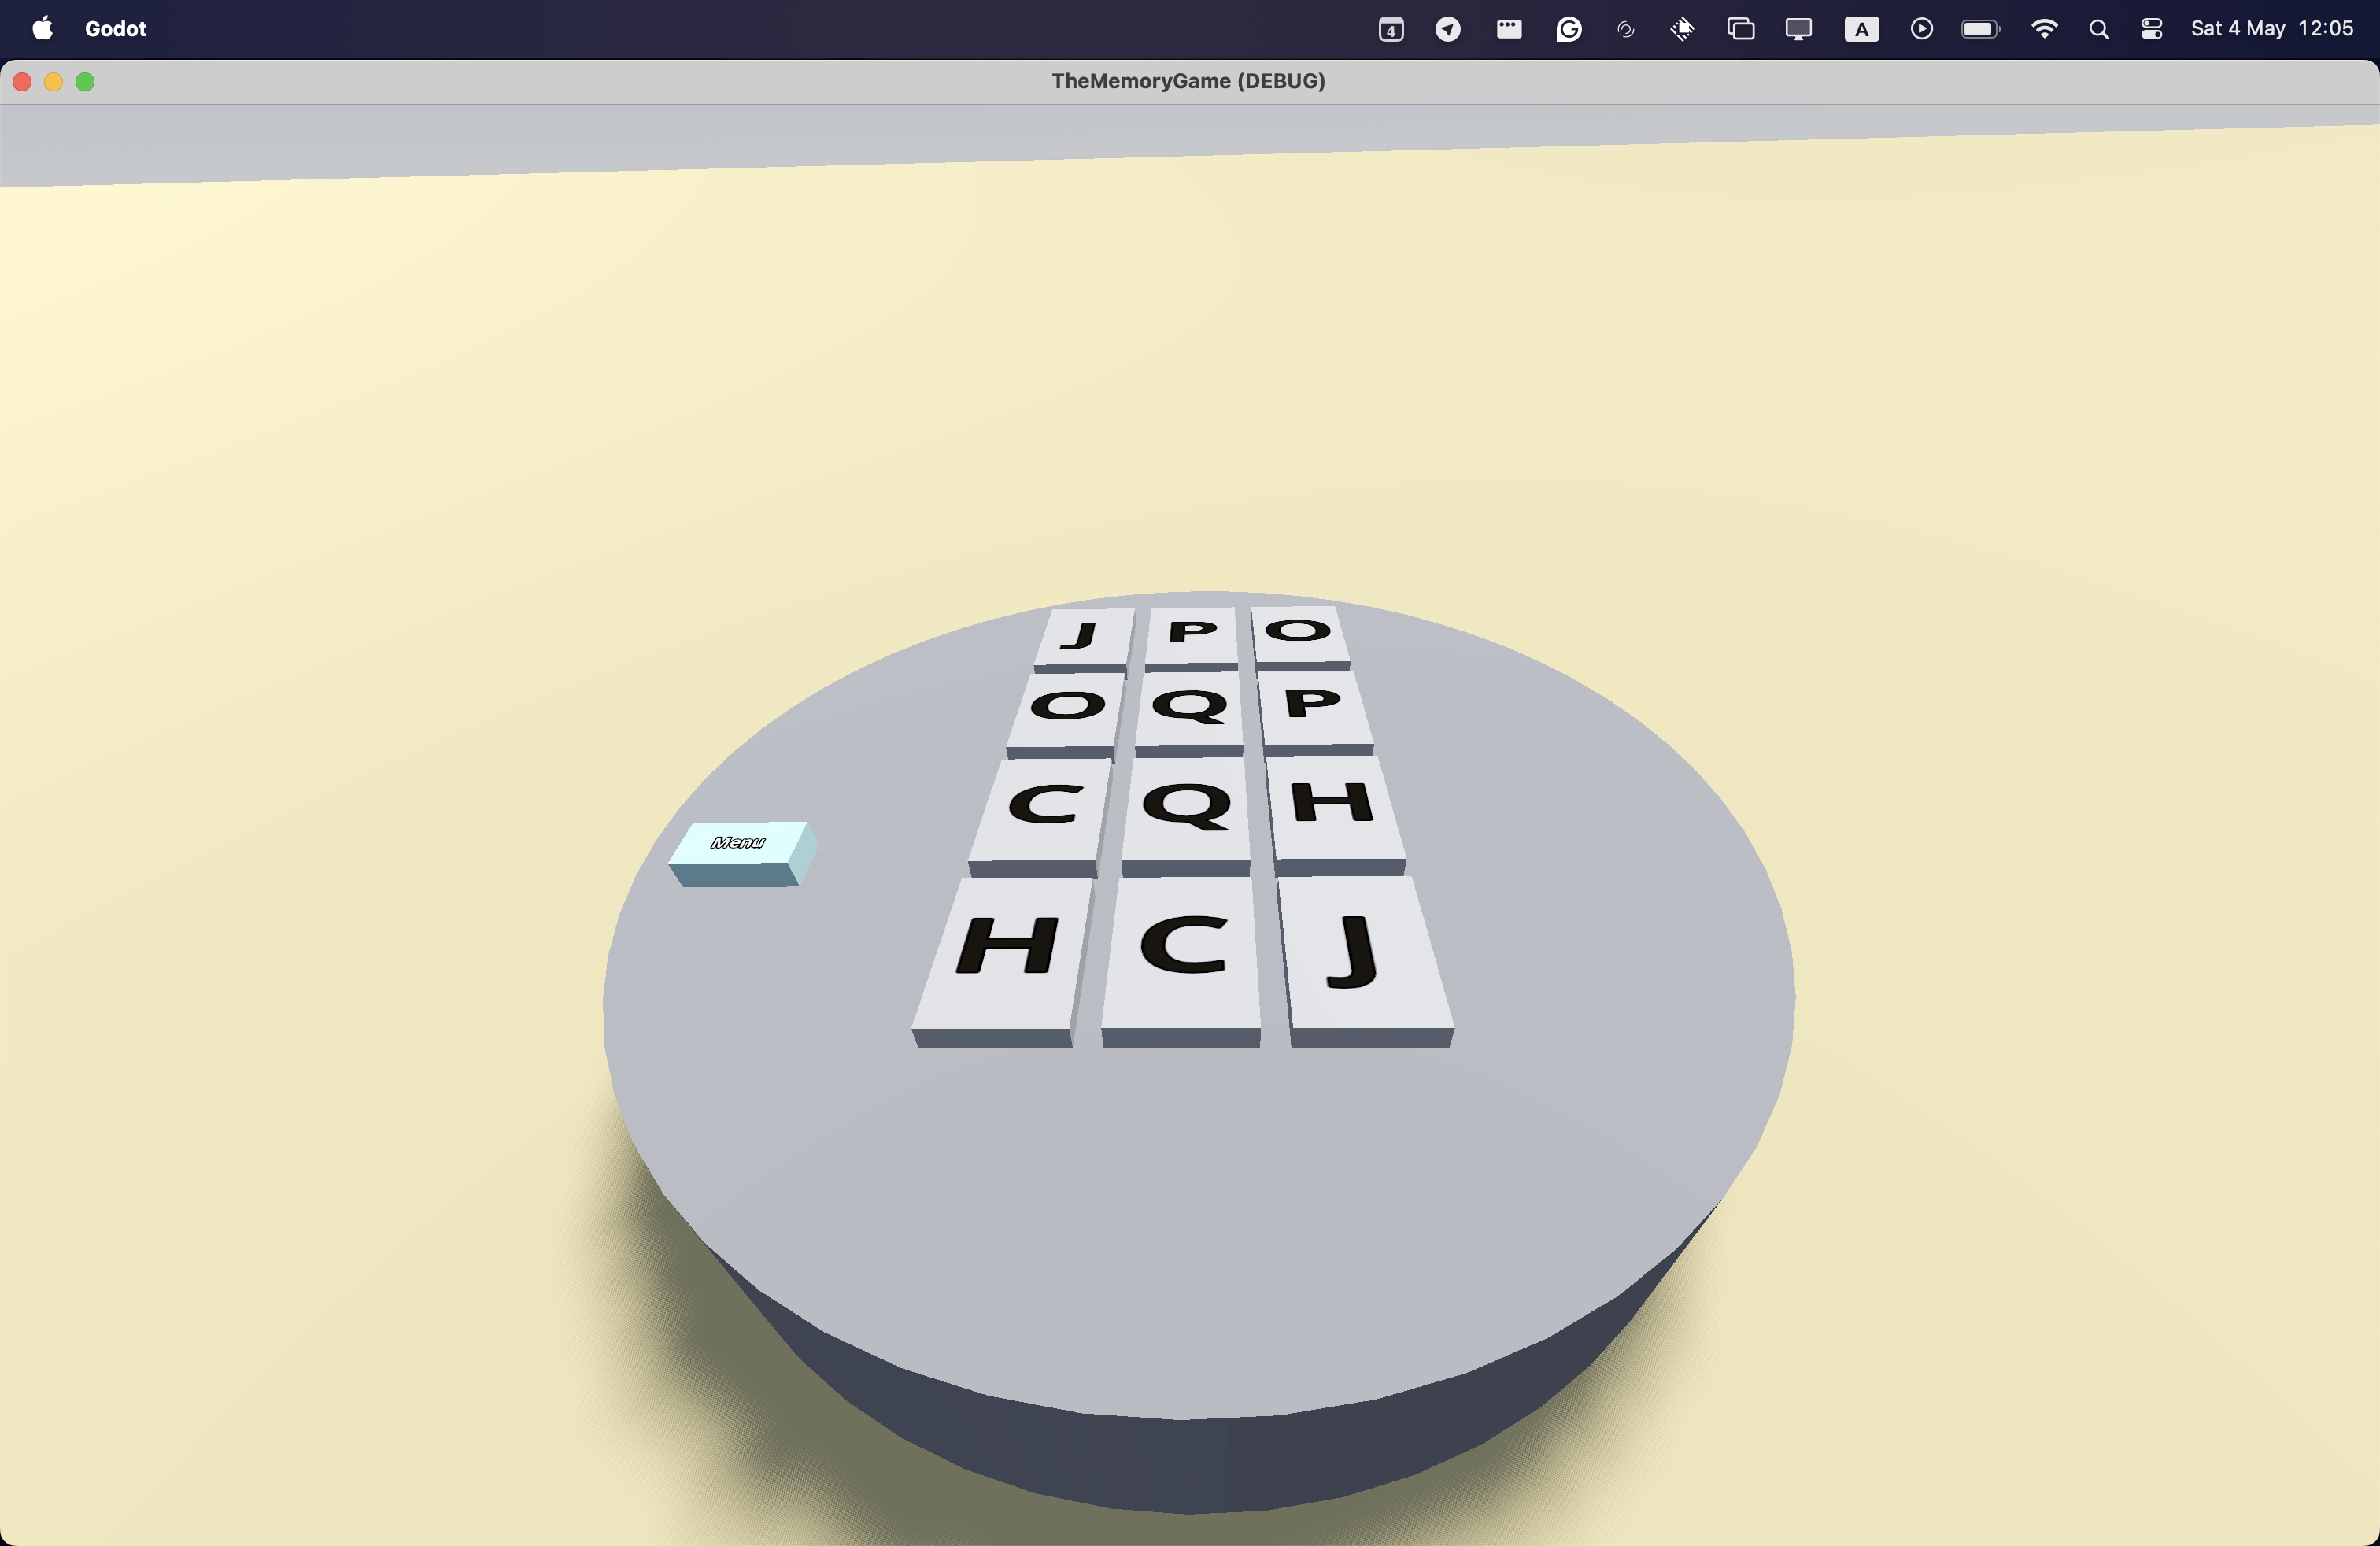
\includegraphics[width=\textwidth]{img/4x4_all_card_fliped.png}
        \caption{4x4 kártya. Minden betűből csak egy pár szerepel}
        \label{img:cards_has_pairs}  
    \end{minipage}
\end{figure}

A kártya rendelkezik animációval is, melyet az AnimationTree (\ref{img:animation_tree}. ábra) kezel. 
Ha rányomunk a kártyára, akkor lefut a \lstinline|card_flip_animation| function, vagyis az AnimationTree State Machine-nek odaadjuk azt az információt, mely szerint meg kell fordítani a kártyát. Az objektum elküldi önmagát a \lstinline|Deck|-nek, mint kiválasztott kártya. 
\begin{figure}[h]
    \centering
    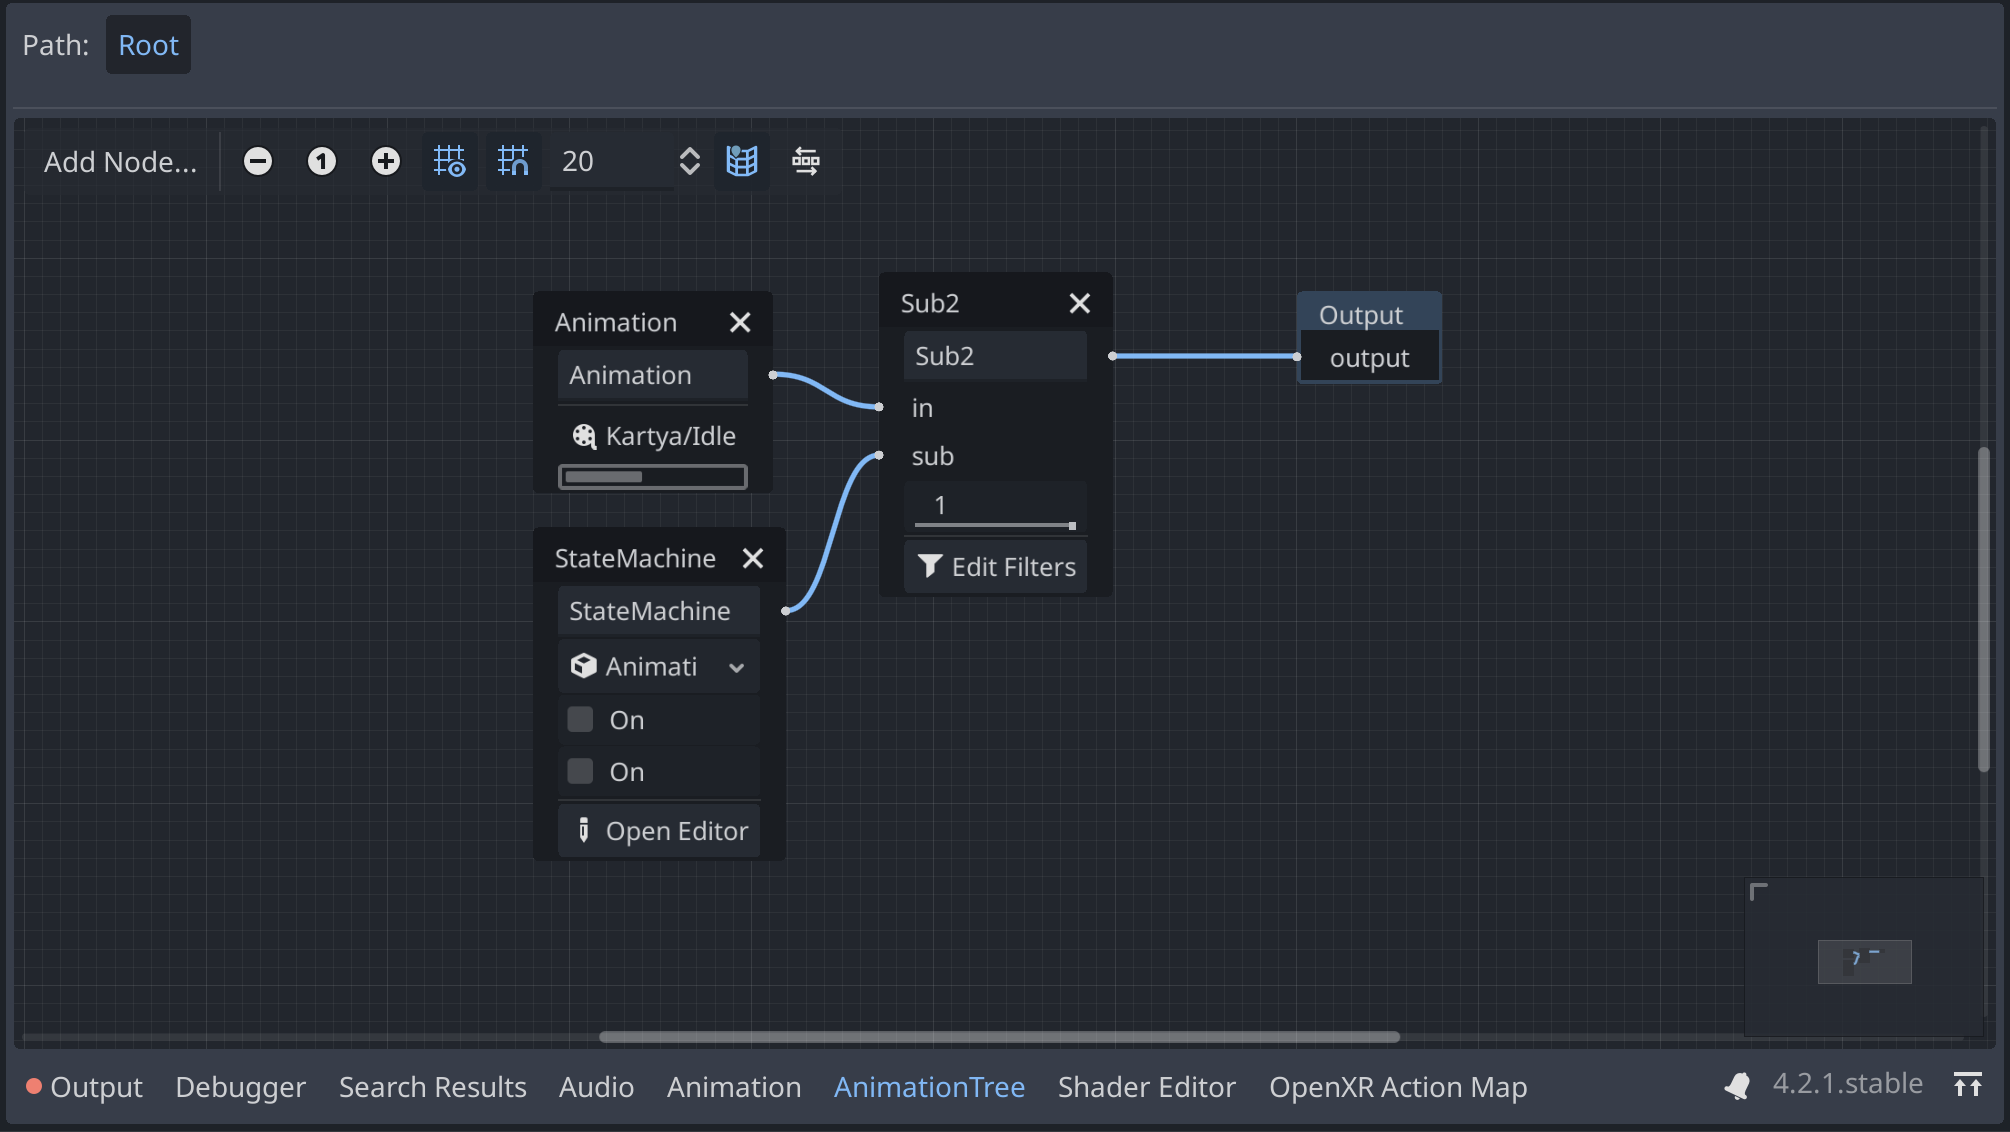
\includegraphics[width=\textwidth]{img/animation_tree.png}
    \caption{A Card animáció fája}
    \label{img:animation_tree}  
\end{figure}




	%\chapter{Összefoglalás}
\thispagestyle{fancy}
\pagestyle{fancy}


\section{Az egyes részfeladatok megvalósításának összefoglalása és értékelése}


	%Irodalomjegyzék generálása a dolgozatba a következő sorok hatására történik, szerkeszteni nem kell. A hivatkozott források gyűjteményét a mybib.bib nevű fájlban kell kialakítani
	\bibliography{mybib}
	\pagestyle{plain}
	\addcontentsline{toc}{chapter}{Irodalomjegyzék}
	%megjelenés sorrendjében építi fel az irodalomjegyzéket
	\bibliographystyle{ieeetr}
	% a következő sor a dolgozat digitális mellékletének a tartalmát csatolja a dolgozathoz, ezt a fájllistát a files.tex fájlban kell megírni
	\chapter{Mellékletek}
\thispagestyle{fancy}
\pagestyle{fancy}

\thispagestyle{fancy}
\pagestyle{fancy}

\subsubsection{Beadott fájlok}
\noindent 3D-memoria-jatek-mestereseges-inteligenciaval mappa (a szoftver fájljai):\\
\begin{tabular}{l l}
    \quad icon.svg  & \quad Godot alapértelmezett ikonja a játékhoz \\ 
    \quad icon.svg.import  & \quad Godot metaadat \\ 
    \quad openxr\_action\_map.tres & \quad OpenXR metaadat \\ 
    \quad project.godot  & \quad Godot projekt fájl \\ 
\end{tabular}
\\\\
\noindent 3D-memoria-jatek-mestereseges-inteligenciaval/Animations mappa (a szoftver animációs fájlok):\\
\begin{tabular}{l l}
    \quad Idle.res  & \quad Kártya animáció \\ 
    \quad Megfordit.res  & \quad Kártya megfordít animáció \\ 
    \quad RESET.res  & \quad Kártya Reset animáció \\
\end{tabular}
\\\\
\noindent 3D-memoria-jatek-mestereseges-inteligenciaval/Scenes mappa (a szoftver jelenetei):\\
\begin{tabular}{l l} 
    \quad MainScrenes  & \quad Fő jelenet\\ 
    \quad MenuScene.tscn  & \quad Főmenü jelenet \\ 
    \quad XrOrigin.tscn  & \quad XR kezdőjelenet \\ 
    \quad button.tscn  & \quad Gomb jelenet \\ 
    \quad plainField.tscn  & \quad Üres tér jelenet \\ 
    \quad plain\_camera.tscn  & \quad Kamera jelenet \\ 
    \quad basics.tscn  & \quad Alapok jelenet \\ 
    \quad Card.gdshader  & \quad Kártya shader\\ 
    \quad Card.tscn  & \quad Kártya jelenet\\ 
    \quad Outline.gdshader  & \quad Kártya körvonal shader\\ 
\end{tabular}

\newpage

\noindent 3D-memoria-jatek-mestereseges-inteligenciaval/Scripts mappa (a szoftver GDScript szkriptjei):\\
\begin{tabular}{l l}
    \quad Card.gd  & \quad Kártya jelenet szkriptje \\ 
    \quad Deck.gd  & \quad Paklik jelenet szkriptje \\ 
    \quad InputField.gd  & \quad Bemeneti mező szkript \\ 
    \quad MenuScene.gd  & \quad Menü jelenet szkriptje \\ 
    \quad VrScript.gd  & \quad VR specifikus szkript \\ 
    \quad basics.gd  & \quad Alap jelent szrikptje \\ 
    \quad button.gd  & \quad Gomb jelent szriptje \\ 
    \quad constant.gd  & \quad Állandók definiálásra használt szkript \\ 
    \quad deck\_timer.gd  & \quad Pakli időzítő szkript \\ 
    \quad http\_client.gd  & \quad HTTP kérések kezelése szkript \\ 
    \quad player\_data.gd  & \quad Játékos adatainak tárolására használt adatszerkezet definiáló szript \\ 
    \quad scene\_manager.gd  & \quad Jelenet váltást kezelő szkript \\ 
\end{tabular}
\\\\
\noindent 3D-memoria-jatek-mestereseges-inteligenciaval/Shaders mappa (A játék grafikai megjelenítését szolgáló fájlok): \\
\begin{tabular}{l l}
    \quad MenuScene.tres  & \quad Menű kinézetét szolgáló shader könyvtár\\ 
    \quad cardTestLibary.tres  & \quad Egy teszt saját shader könyvtár tesztje \\ 
    \quad new\_standard\_material\_3d.tres  & \quad A Gombokhoz használt shader könyvtár \\     
\end{tabular}
\\\\
\noindent 3D-memoria-jatek-mestereseges-inteligenciaval/Templates mappa: \\
\begin{tabular}{l l}
    \quad custom\_build\_template.html  & \quad A HTML exporthoz használt saját html template\\ 
\end{tabular}
\\
\\
\noindent 3D-memoria-jatek-mestereseges-inteligenciaval/fileServer mappa: (Adatok gyüjtését szolgáló fájlszerver) \\
\begin{tabular}{l l}
    \quad Dockerfile  & \quad Docker konténer buildelését szolgáló fájl \\ 
    \quad docker-compose.yaml  & \quad Docker kontérek kezelését szolgáló compose fájl \\ 
    \quad package-lock.json  & \quad Node.JS package-lock fájl, npm használja\\ 
    \quad package.json  & \quad Node.JS package fájl, npm használja. \\ 
    \quad server.js  & \quad Fájlszerver forráskódja \\ 
\end{tabular}

\newpage

\noindent 3D-memoria-jatek-mestereseges-inteligenciaval/tensorflow: (Az MI modell használatához és tanításához szükséges fájlok.) \\
\begin{tabular}{l l}
    \quad json\_to\_sha256.py  & \quad JSON adatok SHA256 konvertálását szolgáló Python szkript \\ 
    \quad my\_model.keras  & \quad A betanított és  mentett MI modell \\ 
    \quad sha256\_to\_binary.py  & \quad SHA256 hash konvertálása bitekre Python szkript \\ 
    \quad tensor.py  & \quad TensorFlow tanító algoritmus, MI betanítása szkript \\ 
    \quad use\_model.py  & \quad Flask szerver, az MI modell használata Python szkript\\ 
\end{tabular}
\\
\\
\noindent SAS\_UEQ mappa (Teszteredmények XLSX fájlai): \\
\begin{tabular}{l l}
    \quad UEQ\_Data\_Analysis\_Tool\_Version12.xlsx & \quad UEQ teszt eredmények XLSX \\
    \quad SAS\_teszt.xlsx & \quad SAS teszt eredmények XLSX \\
\end{tabular}
\\
\\
\noindent p8mqg2\_tex mappa (tex fájlok és képek): \\
\begin{tabular}{l l}
    \quad 4x4\_all\_card\_fliped.png & \quad\quad\quad menu.png\\
    \quad Itch.io.png & \quad\quad\quad menu\_remake.png\\
    \quad JSON.png & \quad\quad\quad menu\_scene\_tree.png\\
    \quad JSON\_TO\_SHA256.png & \quad\quad\quad single\_study\_plot.png\\
    \quad Tensor.png & \quad\quad\quad use\_model.png\\
    \quad UEQ\_diagram.png & \quad\quad\quad Fejezet1.tex\\
    \quad UEQ\_pragmatic\_hedonic.png & \quad\quad\quad Fejezet2.tex\\
    \quad adatgyujtes.png & \quad\quad\quad Fejezet3.tex\\
    \quad allapotgep.png & \quad\quad\quad Fejezet4.tex\\
    \quad animation\_tree.png & \quad\quad\quad Fejezet5.tex\\
    \quad asztal\_4x4.png & \quad\quad\quad Fejezet6.tex\\
    \quad asztal\_4x4\_card\_flipped.png & \quad\quad\quad Fejezet7.tex\\
    \quad asztal\_4x4\_non\_pair.png & \quad\quad\quad Fejezet8.tex\\
    \quad asztal\_4x4\_pair.png & \quad\quad\quad folyamat\_diagram.tex\\
    \quad asztal\_4x4\_pair\_eltunik.png & \quad\quad\quad Abstract.tex\\
    \quad basic\_field\_scene\_structure.png & \quad\quad\quad Fedlap.tex\\
    \quad cards\_scene\_tree.png & \quad\quad\quad Jelolesjegyzek.tex\\
    \quad cloudflair-censored.jpg & \quad\quad\quad Koszonetnyilvanitas.tex\\
    \quad fullfolyamat.jpg & \quad\quad\quad files.tex\\
    \quad fullfolyamat.png & \quad\quad\quad h\_nyilatkozat.tex\\
    \quad hash\_to\_bit.png & \quad\quad\quad tv\_nyilatkozat.tex\\
    \quad kiexportalt.drawio.png & \quad\quad\quad\\
\end{tabular}
\vspace{28pt}


	% a dolgozatban az ábrajegyzéket el kell helyezni, ezt a TeX automatikusan előállítja és a következő sor határása elhelyezi a dokumentumban
	\listoffigures
	%Ha vannak táblázatok is, akkor ezeket is listába gyűjtjük, és a következő utasítással az ábrajegyzéket követően a dolgozatba legeneráltatjuk. Ha nincs rá szükség, a százalék jellel a sor elején érvénytelenítjük a parancsot vagy töröljük a sort
	\listoftables
	
	
\end{document}
